%--beamer--------------------------------------------------------------------------------------
%	PACKAGES AND THEMES
%----------------------------------------------------------------------------------------
\documentclass[xcolor=dvipsnames]{beamer}
\usetheme{default}
\usepackage[backend=bibtex,
defernumbers=true,
style=numeric,
citestyle=ieee
]{biblatex}
\addbibresource{qaref.bib}
\usepackage{hyperref}
\usepackage{graphicx} % Allows including images
\usepackage{booktabs} % Allows the use of \toprule, \midrule and \bottomrule in tables
\usepackage[utf8]{inputenc}
\usepackage[T1]{fontenc}
\usepackage{amsmath,amssymb}
\usepackage{multirow}
\usepackage{array}
\usepackage{pythontex}
\usepackage{hyperref}

% Uncomment here for a Turkish presentation.
%\AtBeginDocument{%
%	\renewcommand\tablename{Tablo}
%}
%\AtBeginDocument{%
%	\renewcommand\figurename{\u015eekil}
%}

%----------------------------------------------------------------------------------------
%	TITLE PAGE
%----------------------------------------------------------------------------------------

% The titlo
\title[Title]
{
 Quantum Algorithms \& Qiskit	
}

\subtitle{}
\author{ Alexander J. Heilman }
 
% can specify the institute here
%\institute[]{\inst{1}Bilgisayar M�hendisli\u011fi B�l�m�\\Gebze Teknik �niversitesi\and\inst{2}Bili\u015fim Teknolojileri Enstit�s�\\Gebze Teknik �niversitesi}

\date{\today} % Date, can be changed to a custom date


%----------------------------------------------------------------------------------------
%	PRESENTATION SLIDES
%----------------------------------------------------------------------------------------

\begin{document}

\begin{frame}
    % Print the title page as the first slide
    \titlepage
\end{frame}


% Uncomment here if you want a table of contents. You should use \section etc. (explained below)
% \begin{frame}{Preface}
%     % Throughout your presentation, if you choose to use \section{} and \subsection{} commands, these will automatically be printed on this slide as an overview of your presentation
%     \tableofcontents
% \end{frame}

%------------------------------------------------

\begin{frame}{Intentions}
    
    Introduce you to some basic quantum algorithms\pause
    \begin{itemize}
        \item Quantum Fourier Transform\pause
        \item Phase Estimation\pause
        \item Amplitude Amplification\pause
    \end{itemize}

    \medskip

    \medskip

    Introduce you to some tools available through Qiskit
    \begin{itemize}
        \item Visualize qubit evolution\pause
        \item Simulate quantum circuits\pause
        \item Experiment with real quantum computers
    \end{itemize}

    \medskip

    \medskip

\center

\pause First, the QFT
\end{frame}

%------------------------------------------------


\center


%------------------------------------------------

\begin{frame}{The Quantum Fourier Transform}
    The quantum Fourier transform (QFT) is a quantum implementation of the discrete
    Fourier transform.

   
    \pause
\begin{columns}
 \column{.42\textwidth}       This means if you give the QFT some basis state $\vert  b \rangle $, the
    QFT will give back states with phases traveling around
    the unit circle at a rate of $\omega ^ b$.\pause
    
  \column{.58\textwidth}   
   
  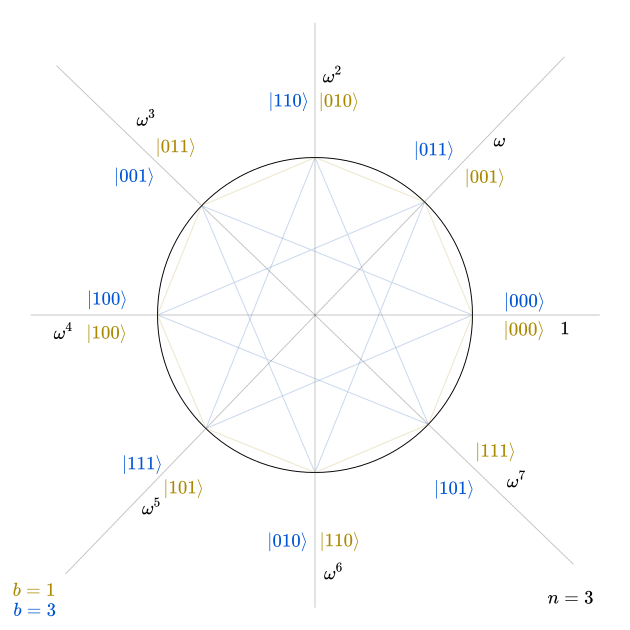
\includegraphics[scale=.4]{qftuc+poly.png}
 
\end{columns}

    \medskip

    \pause

    But how?
\end{frame}

%------------------------------------------------

\begin{frame}{QFT: The gory details}
    The explict action of the n-qubit QFT on some given basis vector is
    
    \vspace{-.7cm}

    \[\hspace{-7cm}
        \vert j_1,...,j_n \rangle  \longrightarrow
    \]

    \vspace{-.9cm}

    \[
        \frac{\left( \vert 0 \rangle  + e^{2\pi i0.j_n} \vert 1 \rangle  \right)\otimes \left( \vert 0 \rangle  + e^{2\pi i0.j_{n-1}j_n} \vert 1 \rangle \right)\otimes ...\otimes \left( \vert 0 \rangle  + e^{2\pi i0.j_1...j_n}  \vert 1 \rangle  \right)  }{2^{n/2} }
    .\] \pause

    \vspace{-.6cm} 
    
    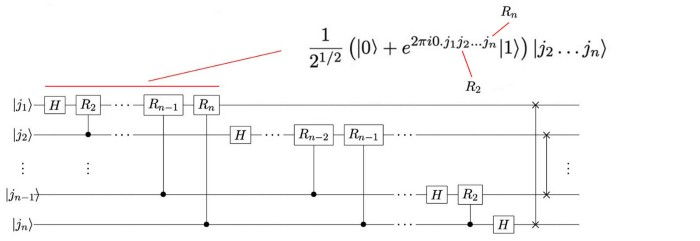
\includegraphics[scale=.51]{nqbqft.jpeg}

    It's easier to see in matrix form
    
    
\end{frame}

%------------------------------------------------

\begin{frame}{QFT: The gory details II}
 For $n=3$ the QFT is 

    
    \[
      \frac{1}{2\sqrt{2}} 
    \begin{bmatrix}
    1 & 1 & 1 & 1 & 1 & 1 & 1 & 1\\
    1 & \omega &\omega ^2      &\omega ^3  &\omega ^{4} &\omega ^{5} &\omega ^{6} &\omega ^{7}\\
    1 & \omega ^2&\omega ^{4}  &\omega^{6} &1       &\omega ^2&\omega ^{4} &\omega ^{6}\\
    1 &\omega ^{3}&\omega ^{6} &\omega     &\omega ^{4} &\omega ^{7} &\omega ^2&\omega ^{5} \\
    1 &\omega ^{4}&           1&\omega^{4} &1&\omega ^{4} &1 & \omega ^{4}   \\
    1 &\omega ^{5}&\omega ^{2} &\omega^{7} &\omega ^{4} &\omega &\omega ^6&\omega ^{3} \\
    1 &\omega ^{6}&\omega ^{4} &\omega^2  &1&\omega ^{6} &\omega ^4&\omega ^{2} \\
    1 &\omega ^{7}&\omega ^{6} &\omega^{5}  &\omega ^{4} &\omega ^{3} &\omega ^2&\omega  \\
\end{bmatrix}
    .\]\pause

    Not so interesting yet, but it's usefulness will soon be found in phase estimation
    
    
\end{frame}

%------------------------------------------------

\begin{frame}{Phase Estimation}
	Phase Estimation takes some given unitary operator and an associated eigenvector
    and returns the corresponding eigenvalue.

    
    \[
        \text{If } U\vert\psi\rangle  = \lambda\vert\psi\rangle \quad\text{ then }\quad U,\vert \psi  \rangle 
        \overset{PE} \longrightarrow\lambda   
    \].\pause 
    
    

    \medskip

    Really it returns $\vert k \rangle $, where the eigenvalue is $\lambda = e^{i\theta }$
    with $\theta =k \frac{2\pi }{2^{n} } $. \pause (Or closest n-bit approx. with at least 40\% probability)

    \medskip\pause

    So how do we do this? \pause Easy!
\end{frame}

%------------------------------------------------

%------------------------------------------------

\begin{frame}{Phase Estimation: Not so bad!}
       
   \begin{figure}
    \begin{overprint}
        \onslide<1>\centering\vspace{.3cm}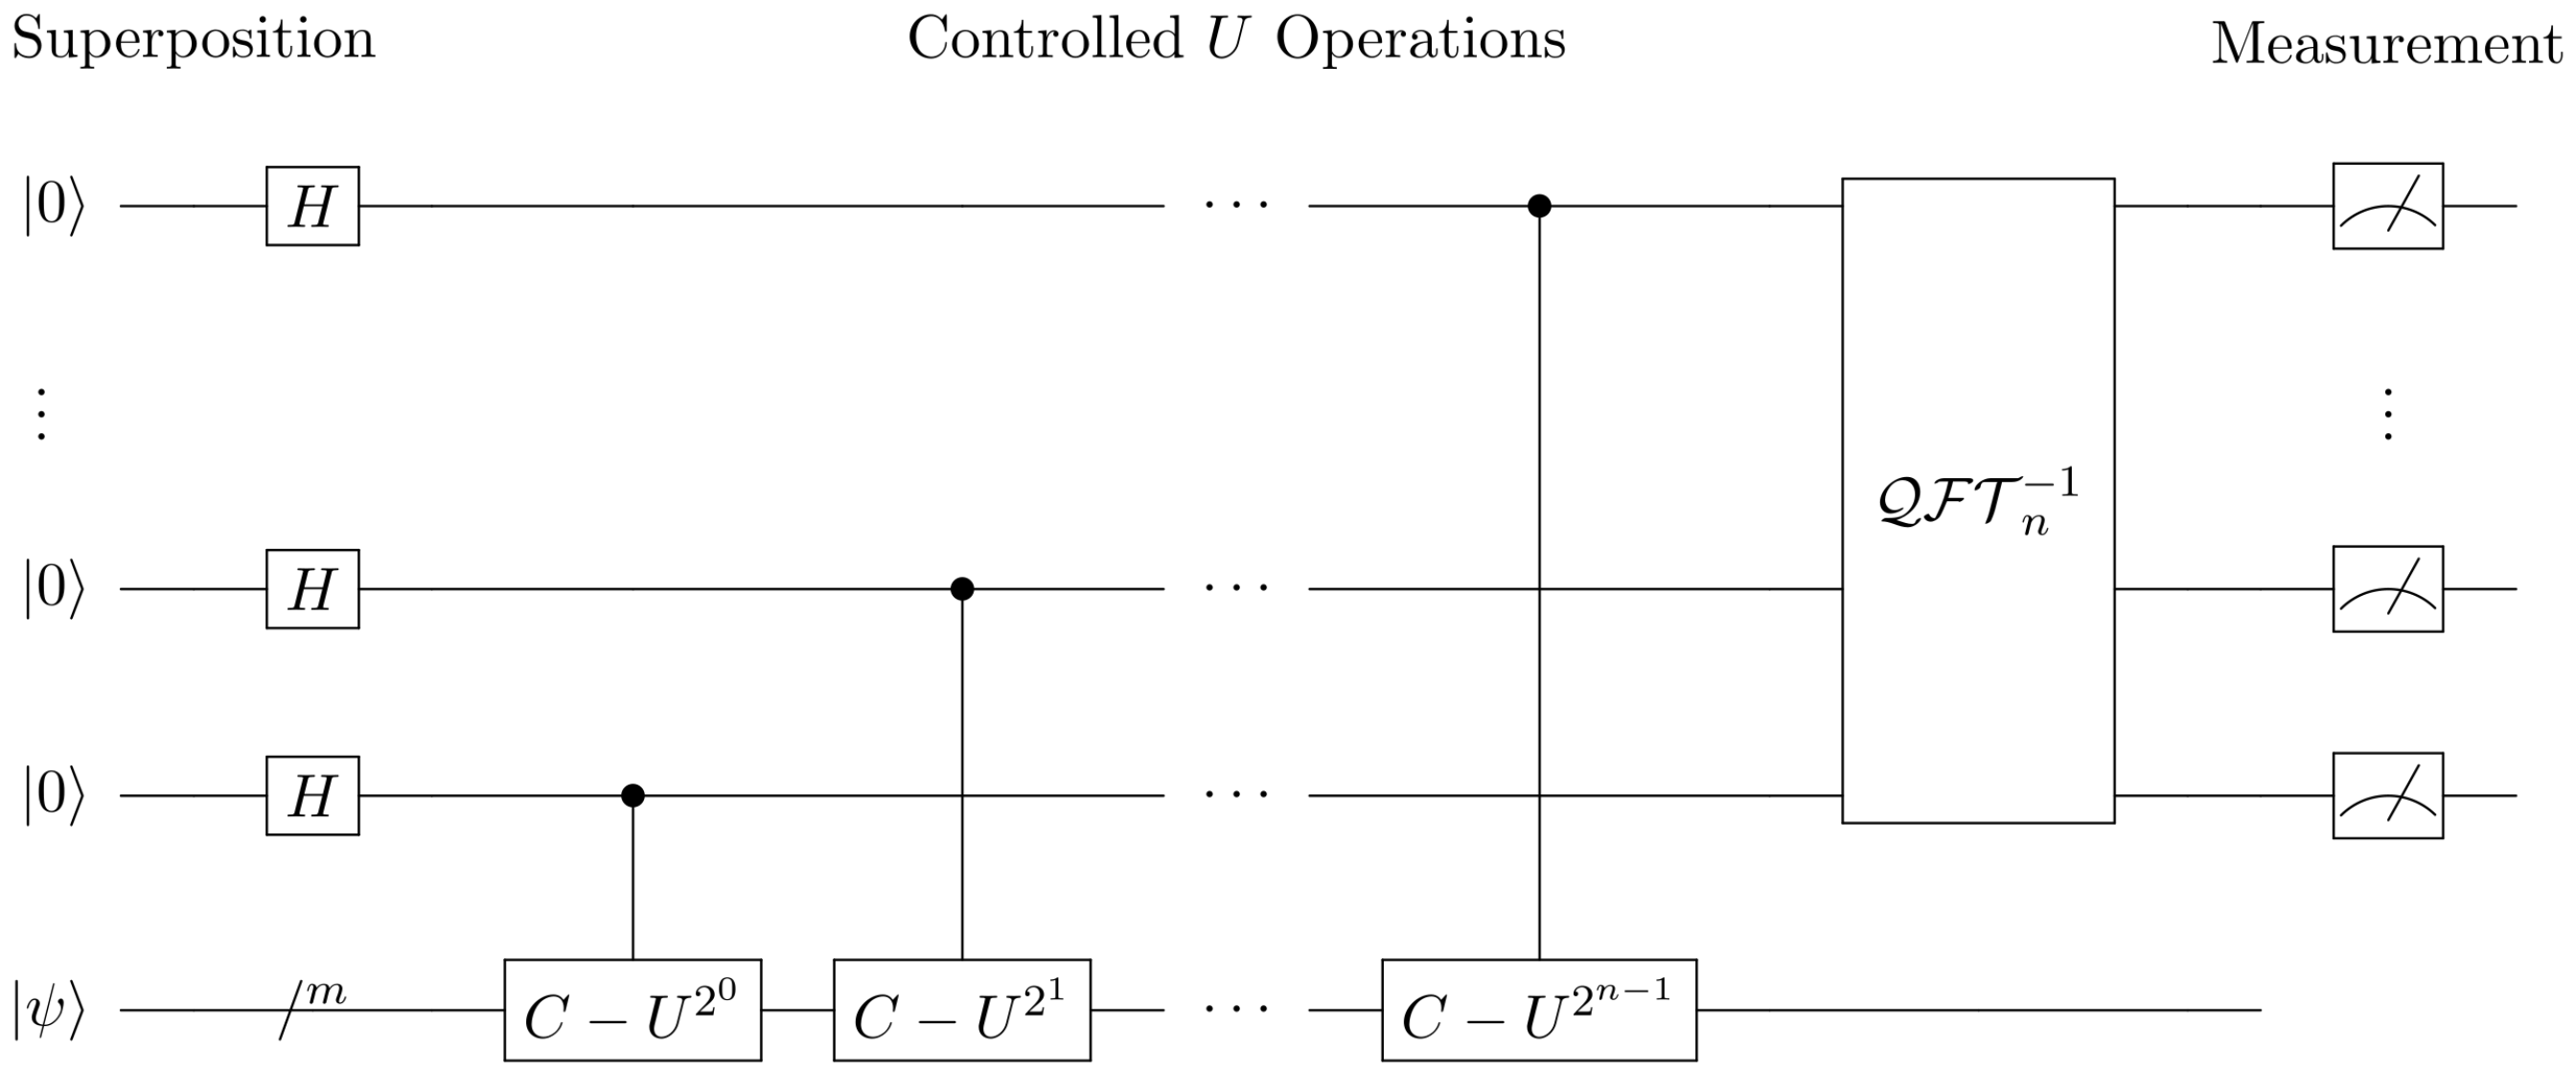
\includegraphics[scale=.15]{nqubitpe.png}
        \onslide<2>\centering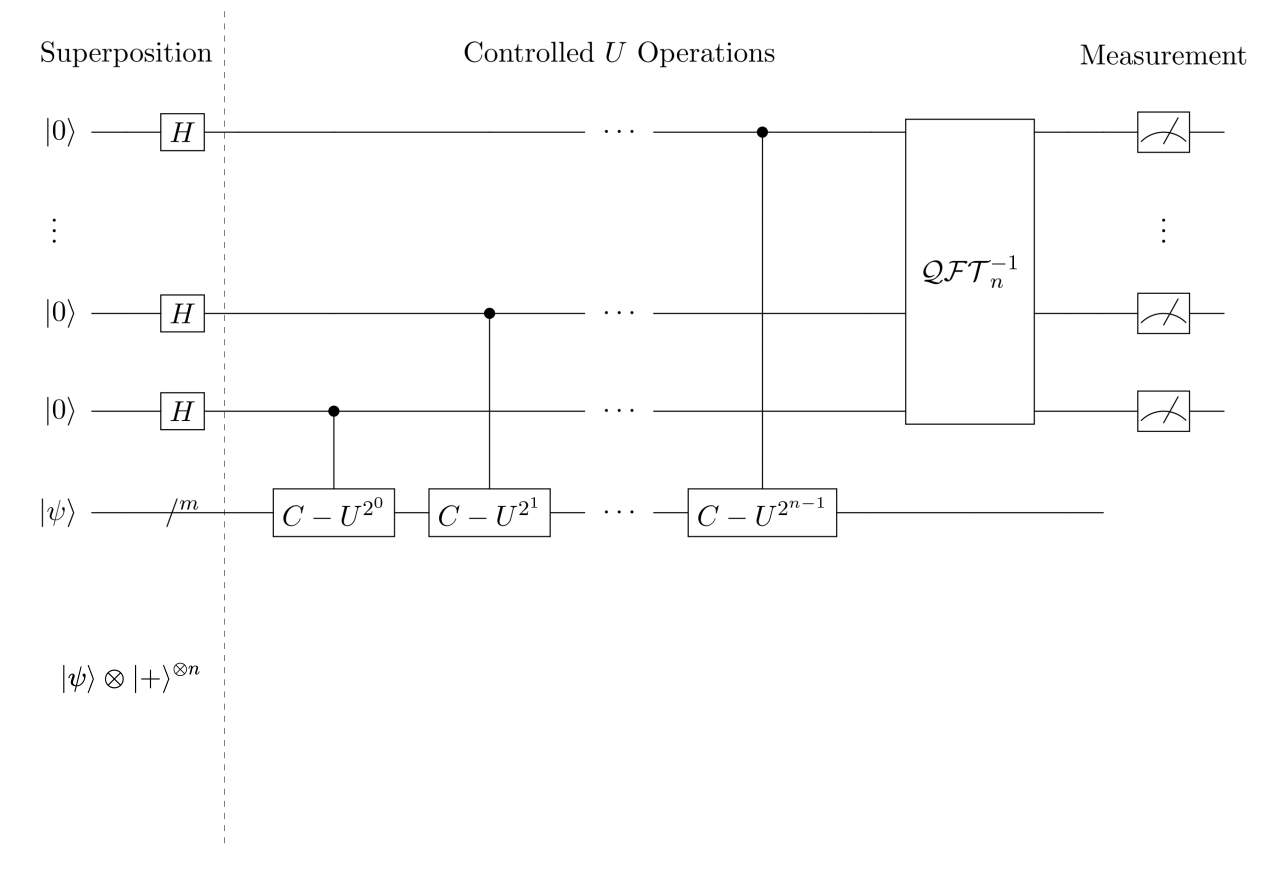
\includegraphics[scale=.33]{nqubitpemu1.png}
        \onslide<3>\centering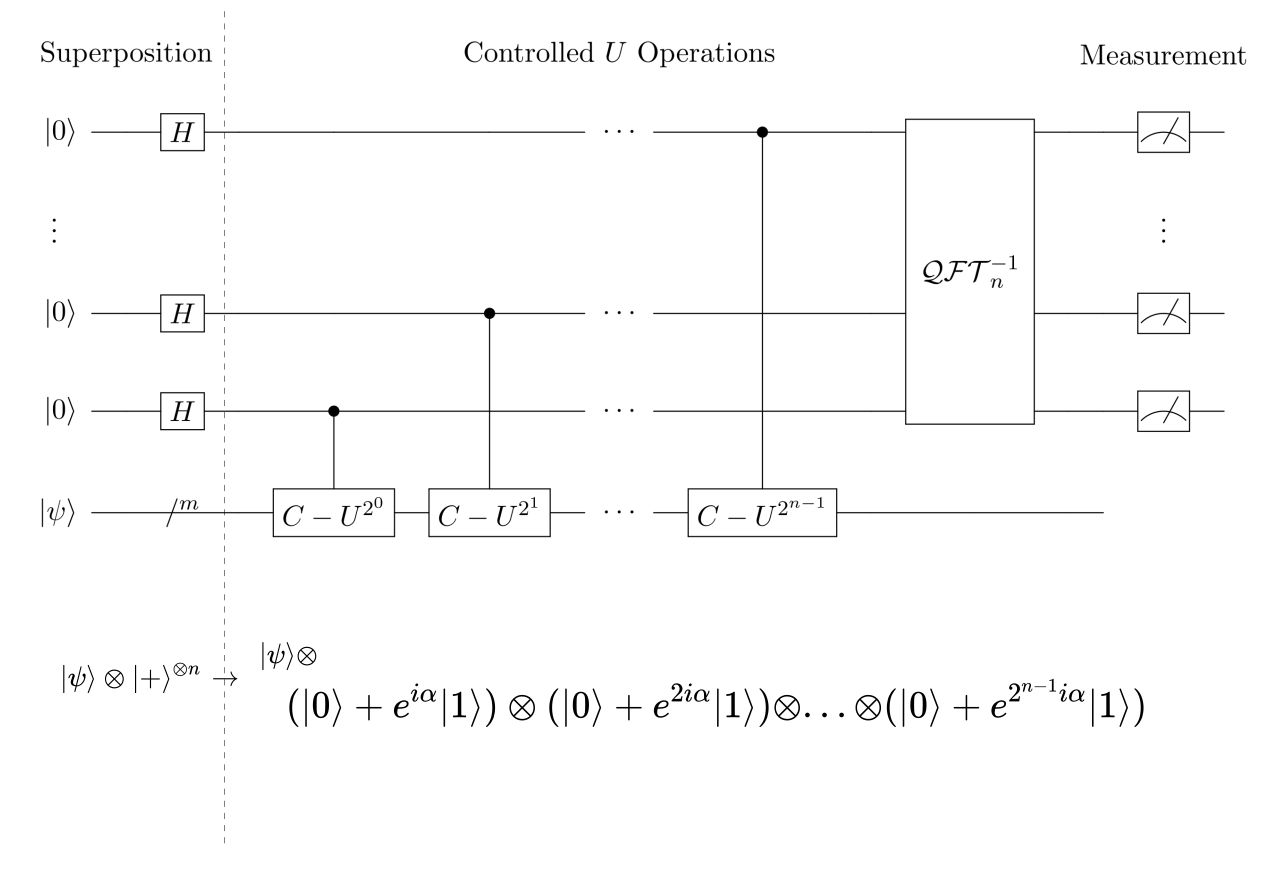
\includegraphics[scale=.33]{nqubitpemu2.png}
        \onslide<4>\centering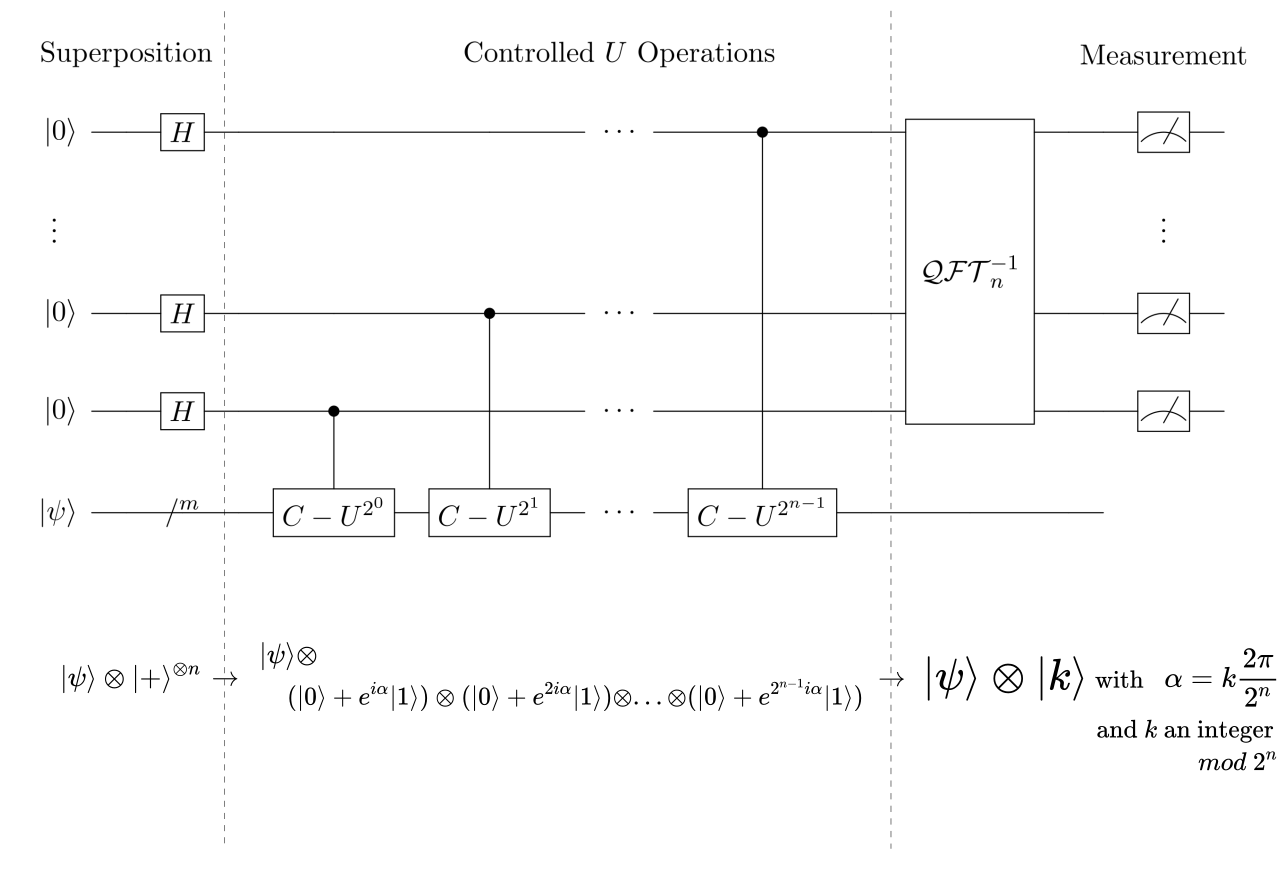
\includegraphics[scale=.33]{nqubitpemu3.png}
    \end{overprint}
\end{figure}


\end{frame}

%------------------------------------------------

%------------------------------------------------

\begin{frame}{Amplitude Amplification}
    Amplitude estimation takes some statevector partitioned into a 
    good and a bad subspace
    
    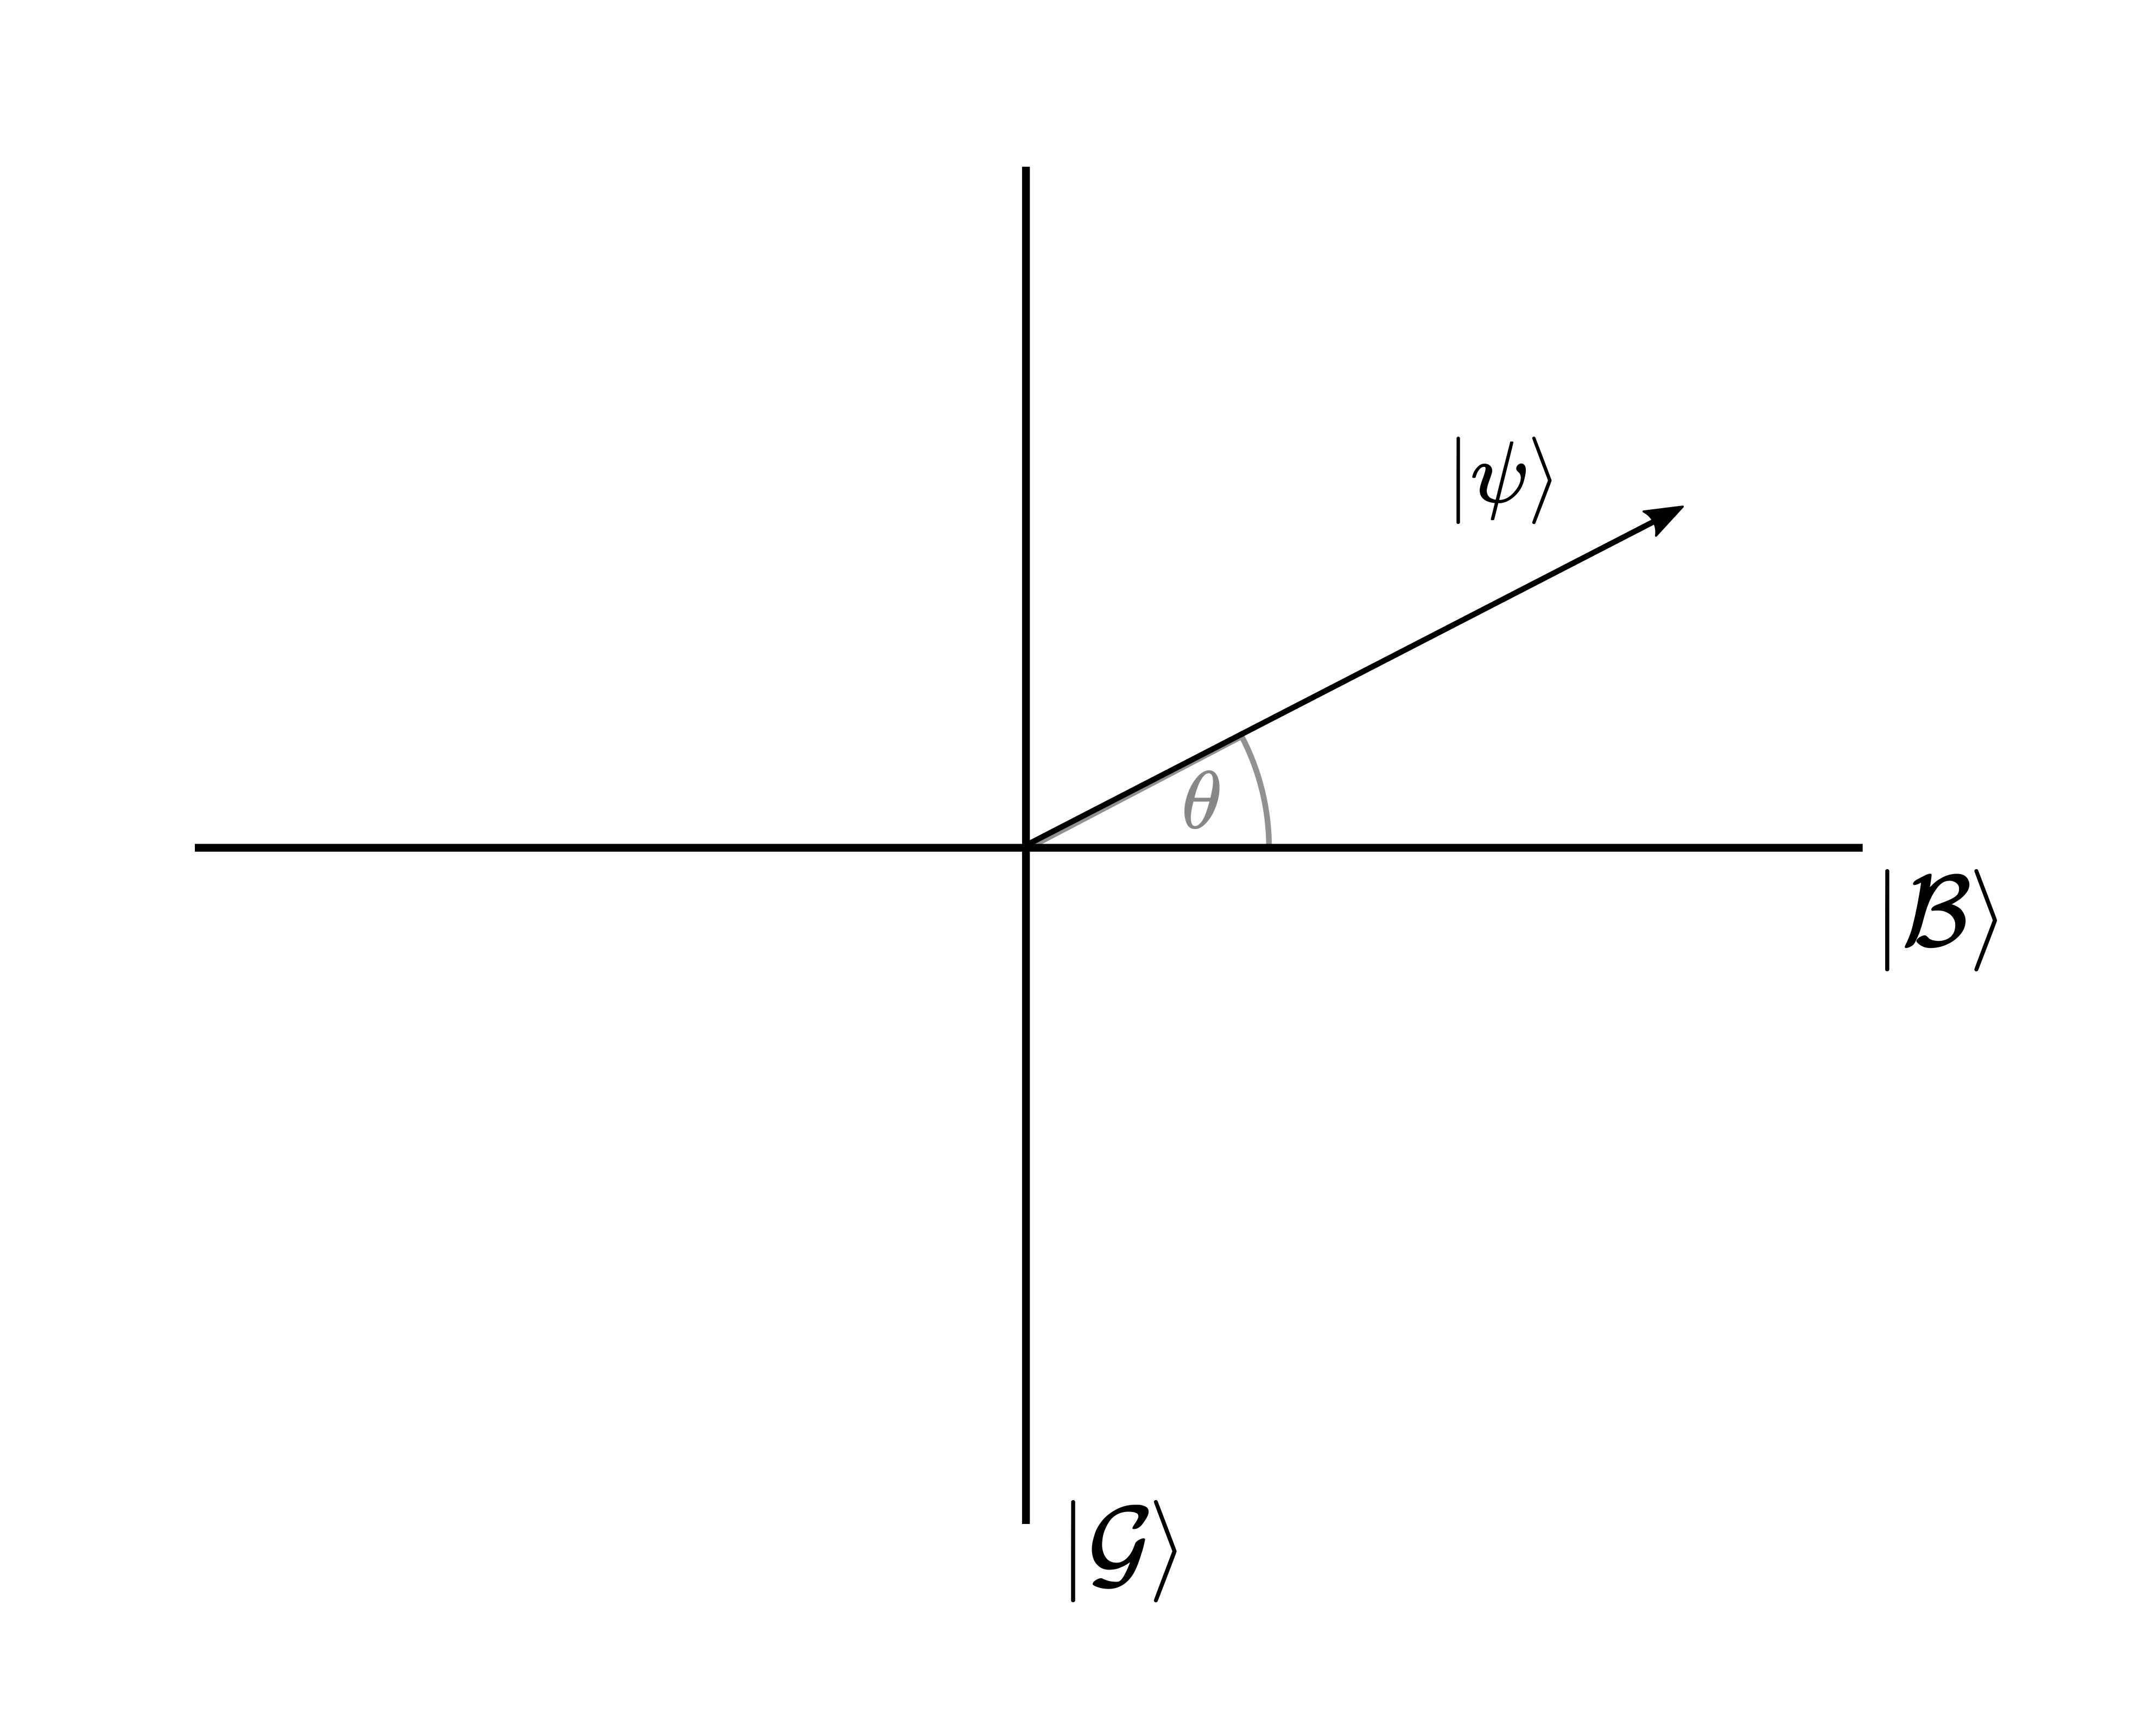
\includegraphics[scale=.7]{psi.png}\pause

     $\vert \psi  \rangle = sin(\theta )\vert \mathcal{G} \rangle +cos(\theta ) \vert \mathcal{B} \rangle  $.


\end{frame}

%------------------------------------------------

%------------------------------------------------

\begin{frame}{Amplitude Amplification}

    And returns a statevector nudged towards the good subspace.

    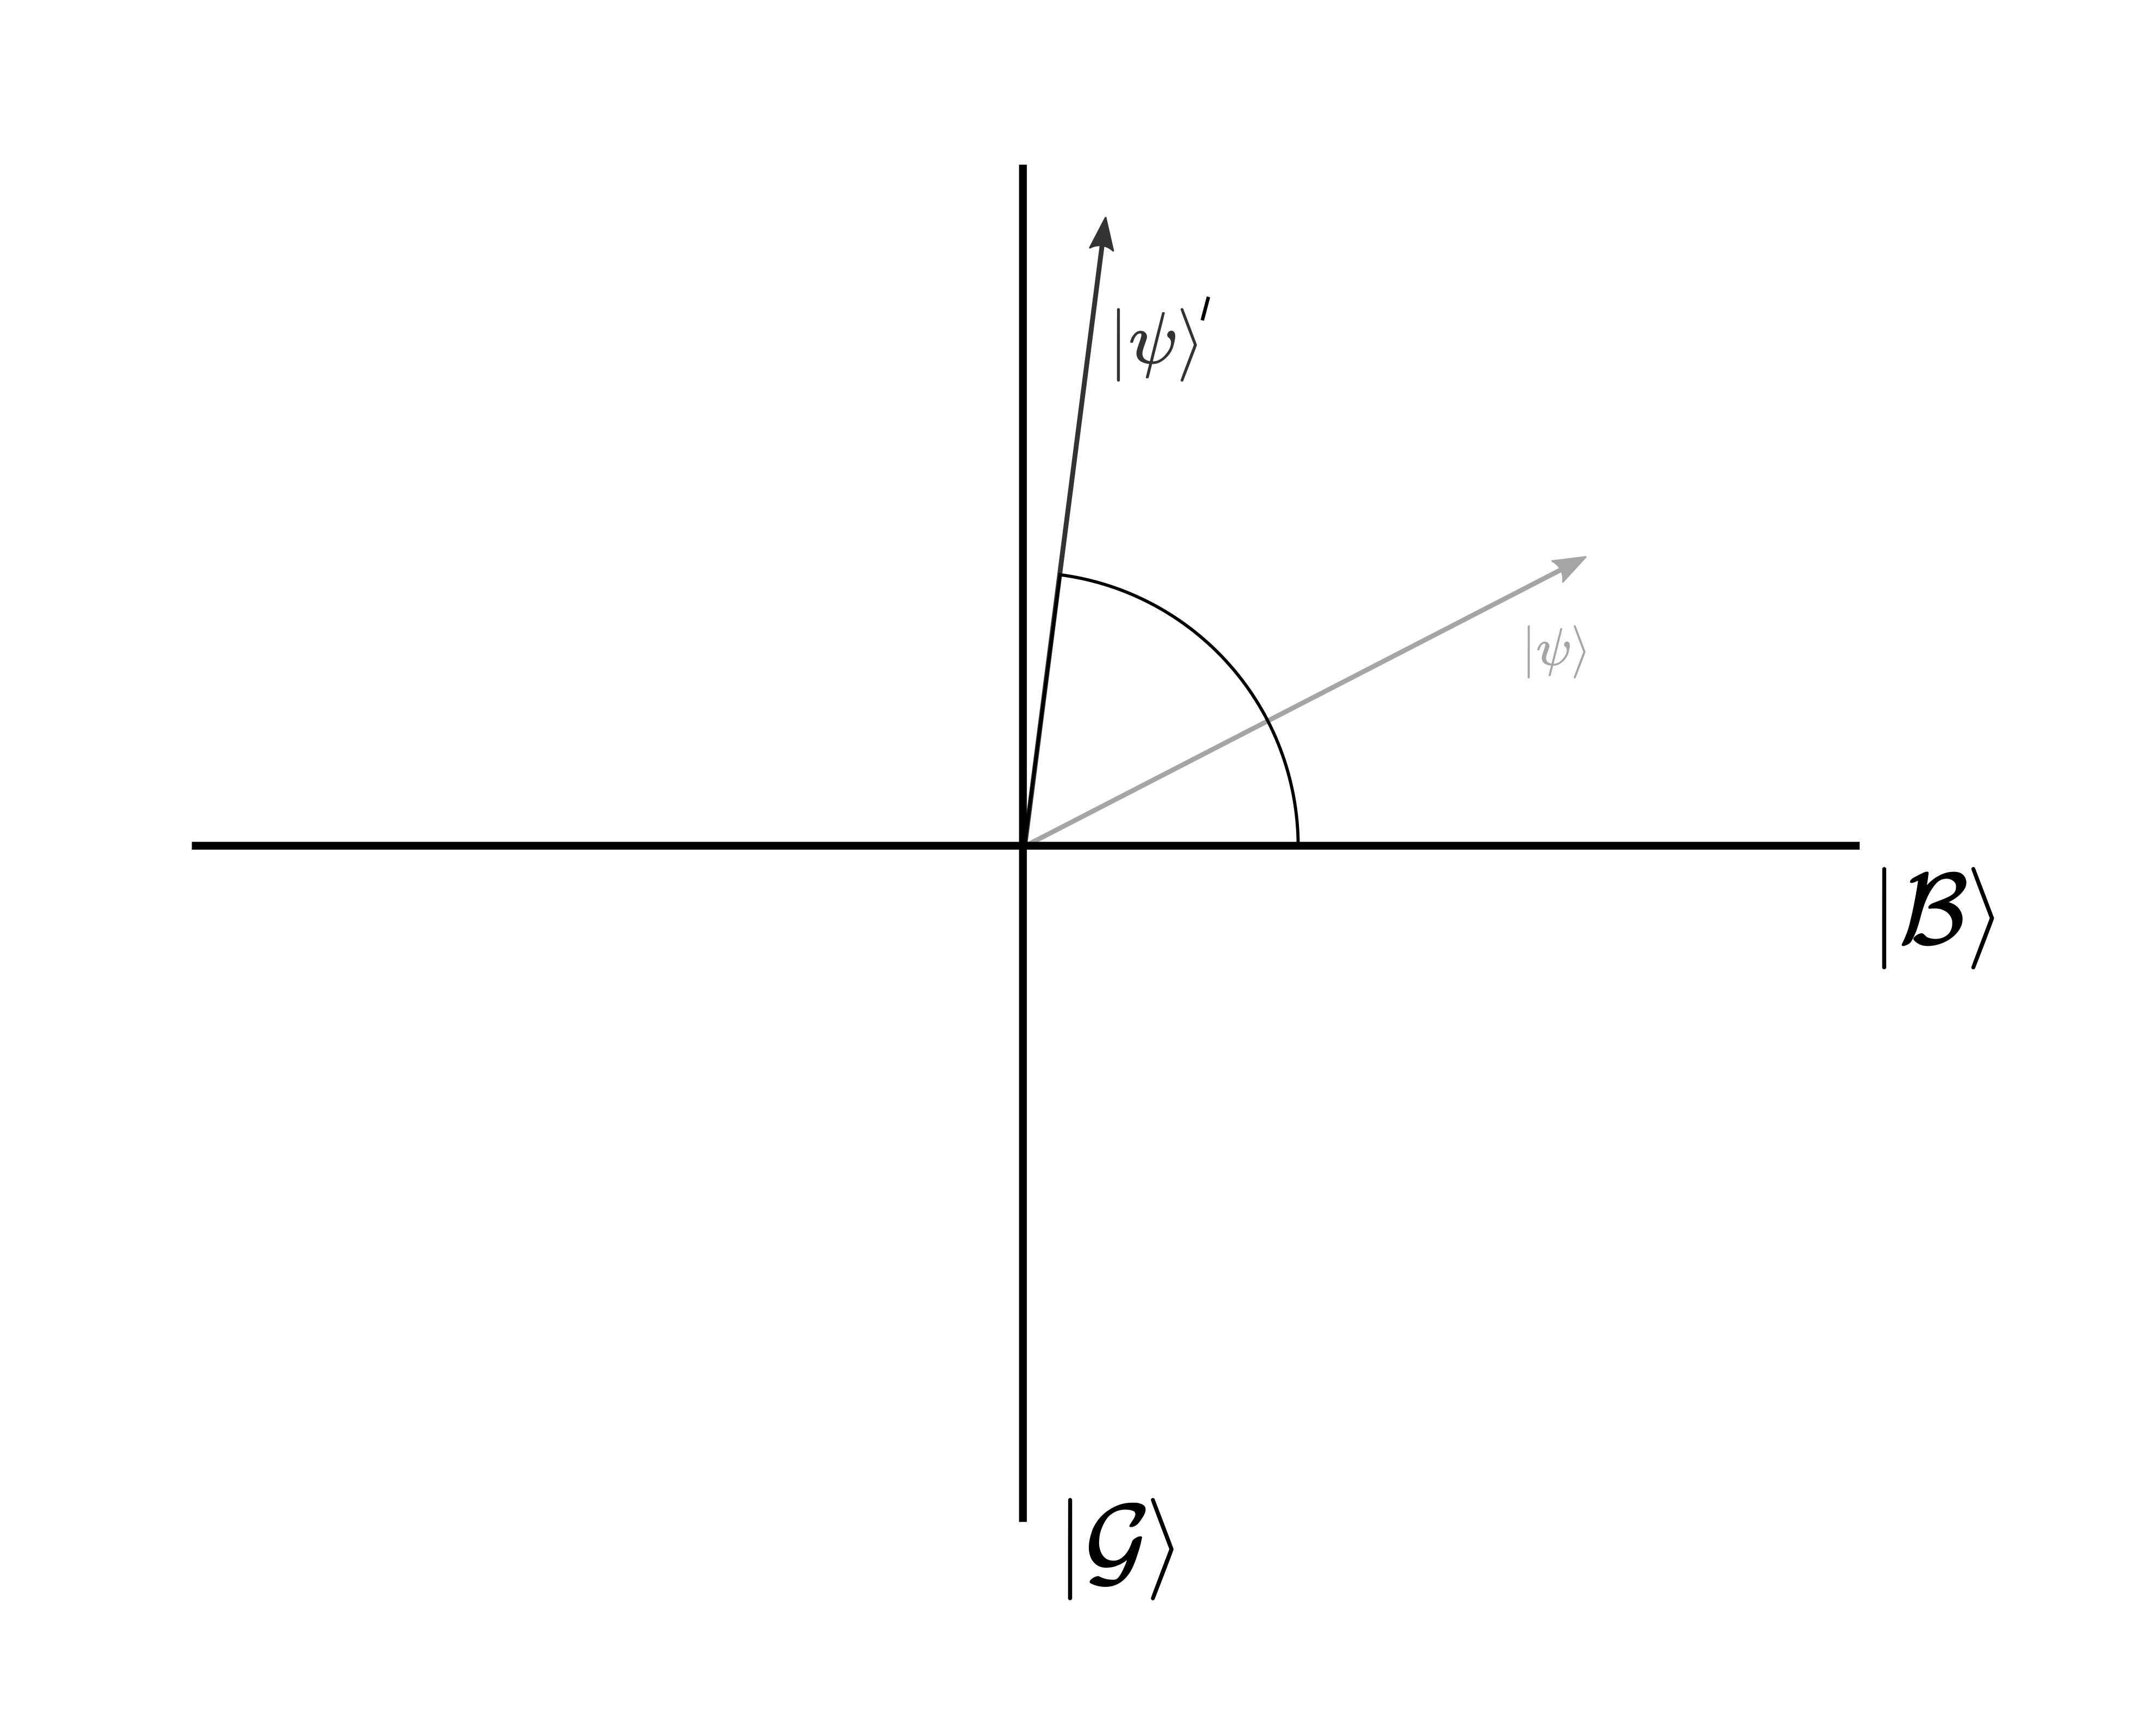
\includegraphics[scale=.7]{psinudge.png}\pause

    This is accomplished with consecutive applications of a special operator 
\end{frame}

%------------------------------------------------


%------------------------------------------------

\begin{frame}{Amplitude Amplification: Working principles}
    Remember $\vert \psi  \rangle = sin(\theta )\vert \mathcal{G} \rangle +cos(\theta ) \vert \mathcal{B} \rangle  $.\pause

    \medskip
    
  	\begin{columns}[c] % The "c" option specifies centered vertical alignment while the "t" option is used for top vertical alignment
		

	    \column{.15\textwidth}	
		\column{.35\textwidth} % Right column and width
          We define operators:\pause
		\column{.55\textwidth} % Left column and width
		\begin{enumerate}
            \item \( \mathcal{S}_{\mathcal{G}}
                                           =\mathbb{I}-2\vert \mathcal{G} \rangle
                                           \langle \mathcal{G} \vert \)\pause
            \item  \( \mathcal{S}_{\psi}
                                         =\mathbb{I}-2\vert \psi
                                         \rangle\langle\psi \vert \)\pause

            \item  \( \mathcal{Q}=-\mathcal{S}_{\psi}\mathcal{S}_{\mathcal{G}}\)
		\end{enumerate}
	\end{columns}\pause

    \vspace{1.3cm}

    Let's see what they do!
\end{frame}

%------------------------------------------------

\begin{frame}{Amplitude Amplification: Visualization I}

    First apply the operator $ \mathcal{S}_{\mathcal{G}} $,

   \begin{figure}
    \begin{overprint}
        \onslide<1>\centering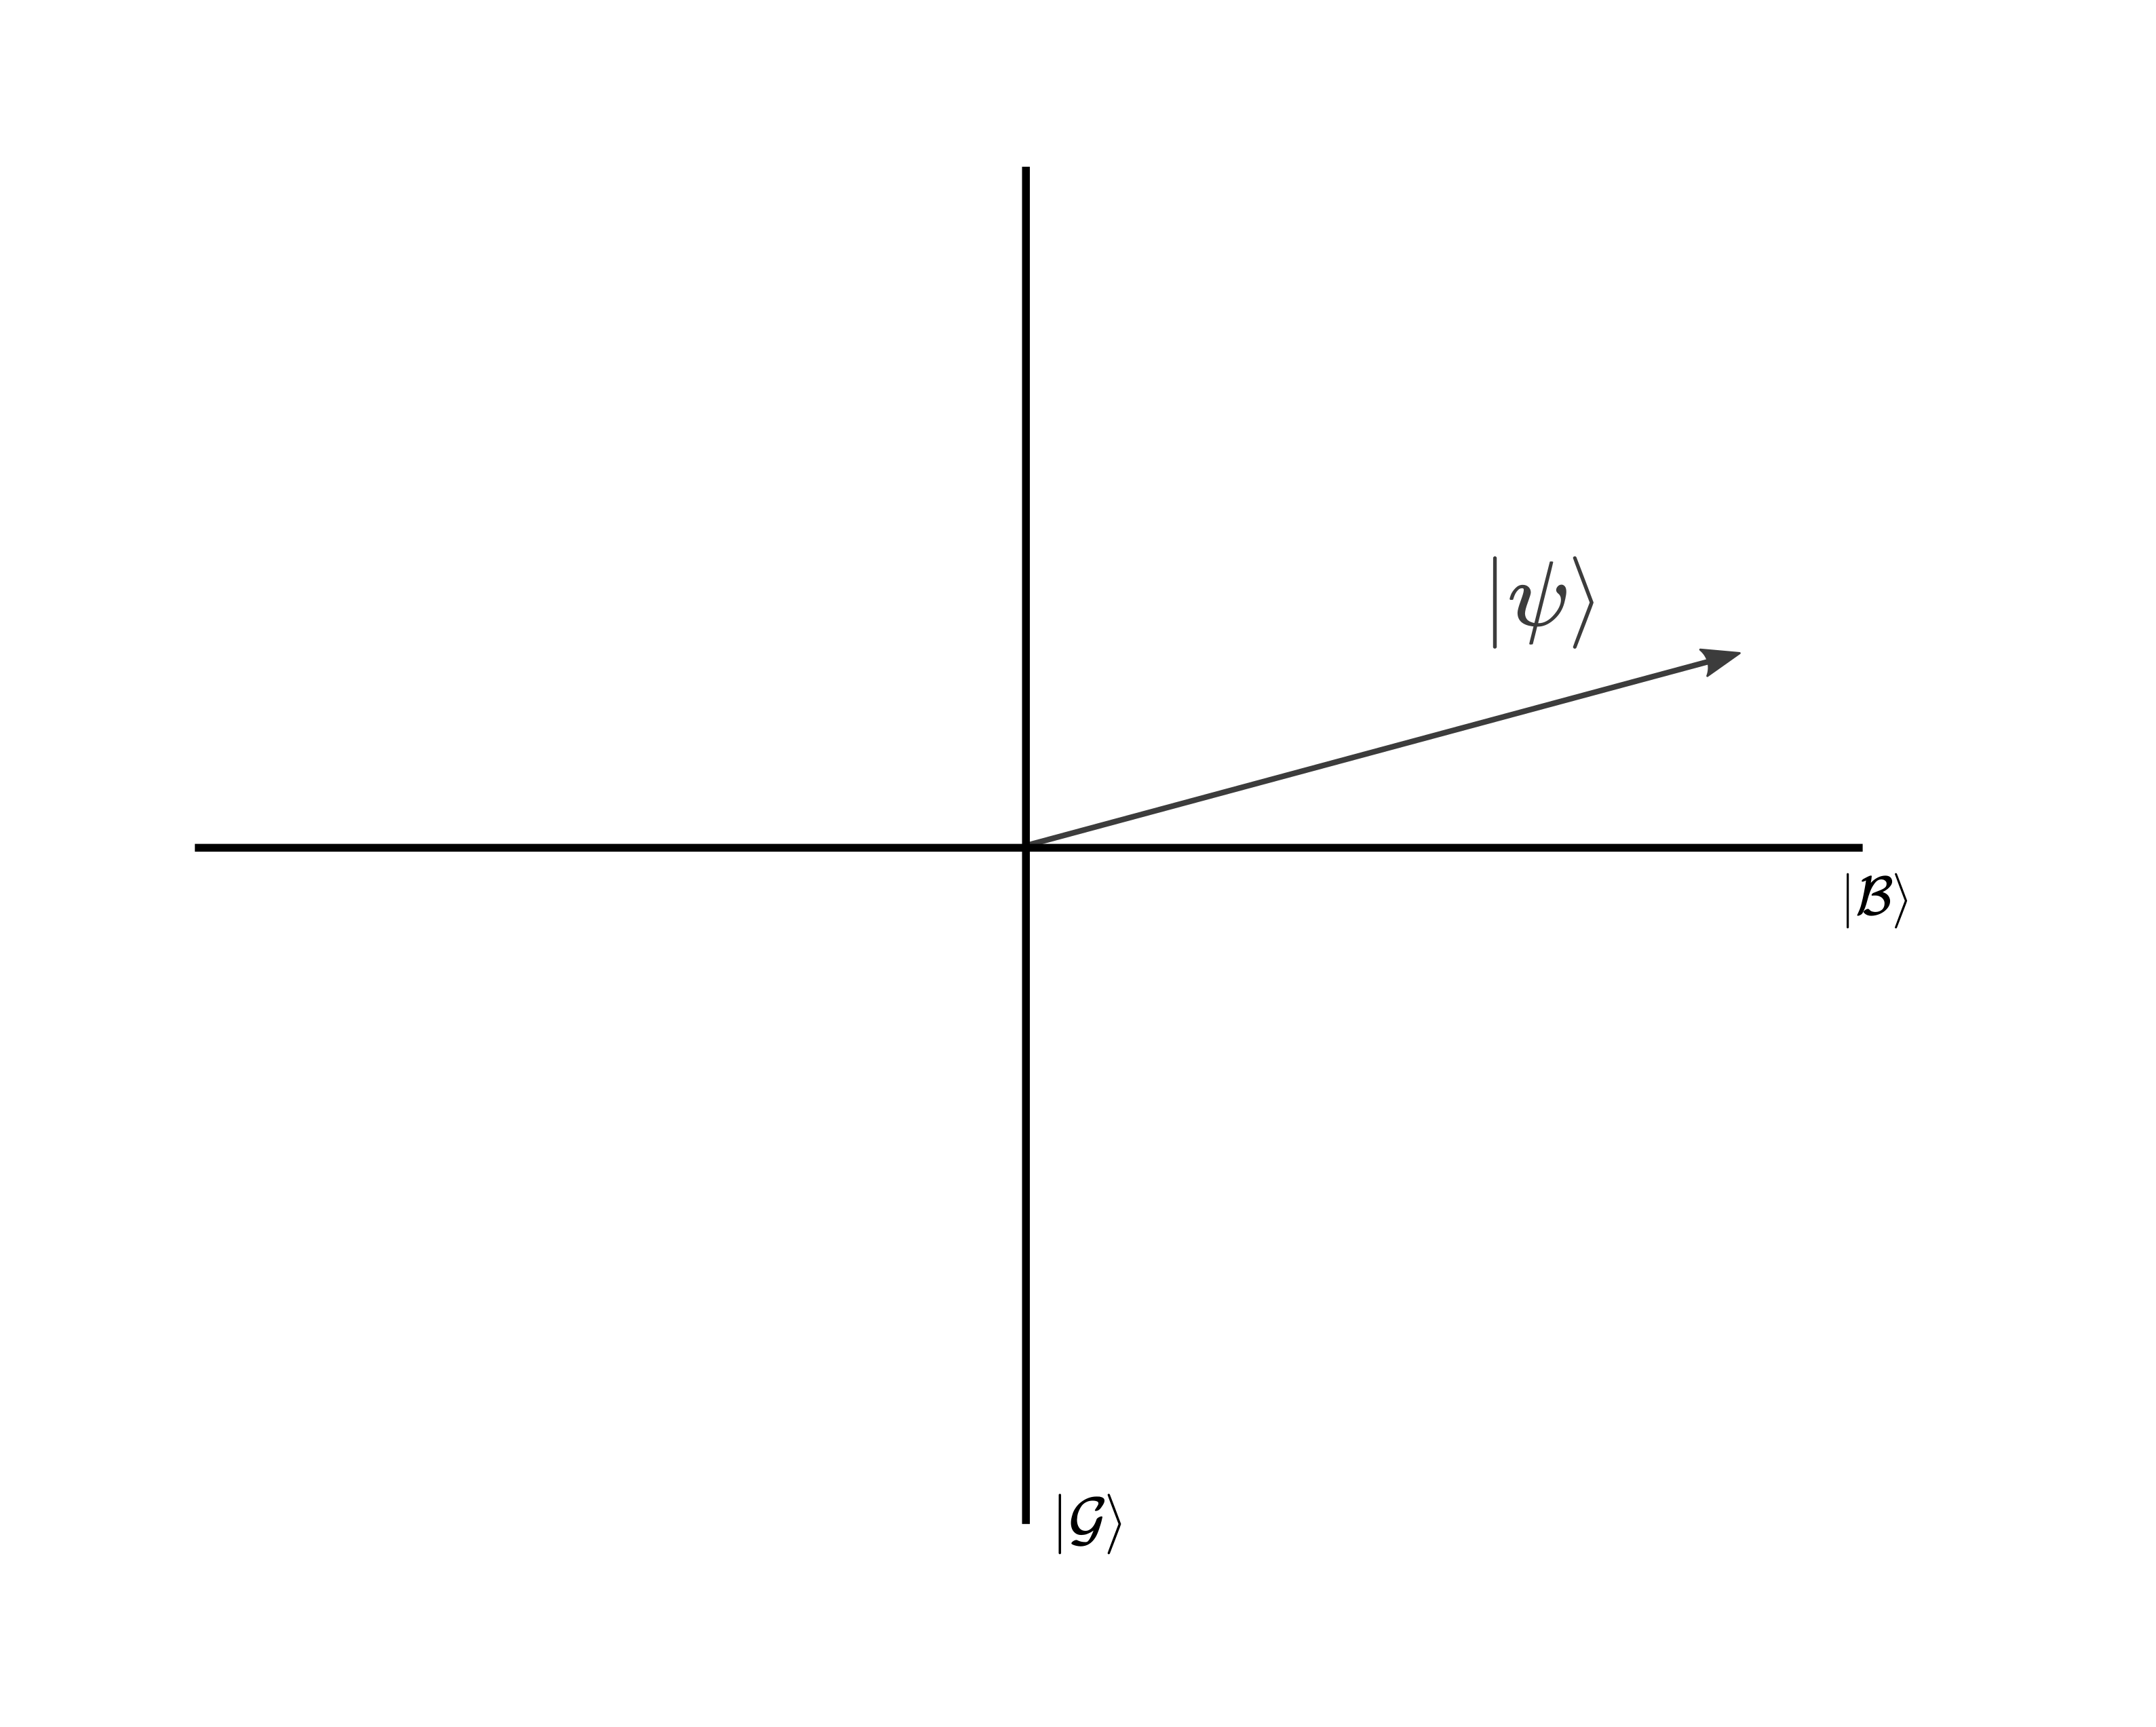
\includegraphics[scale=.87]{psi4.png}
        \onslide<2>\centering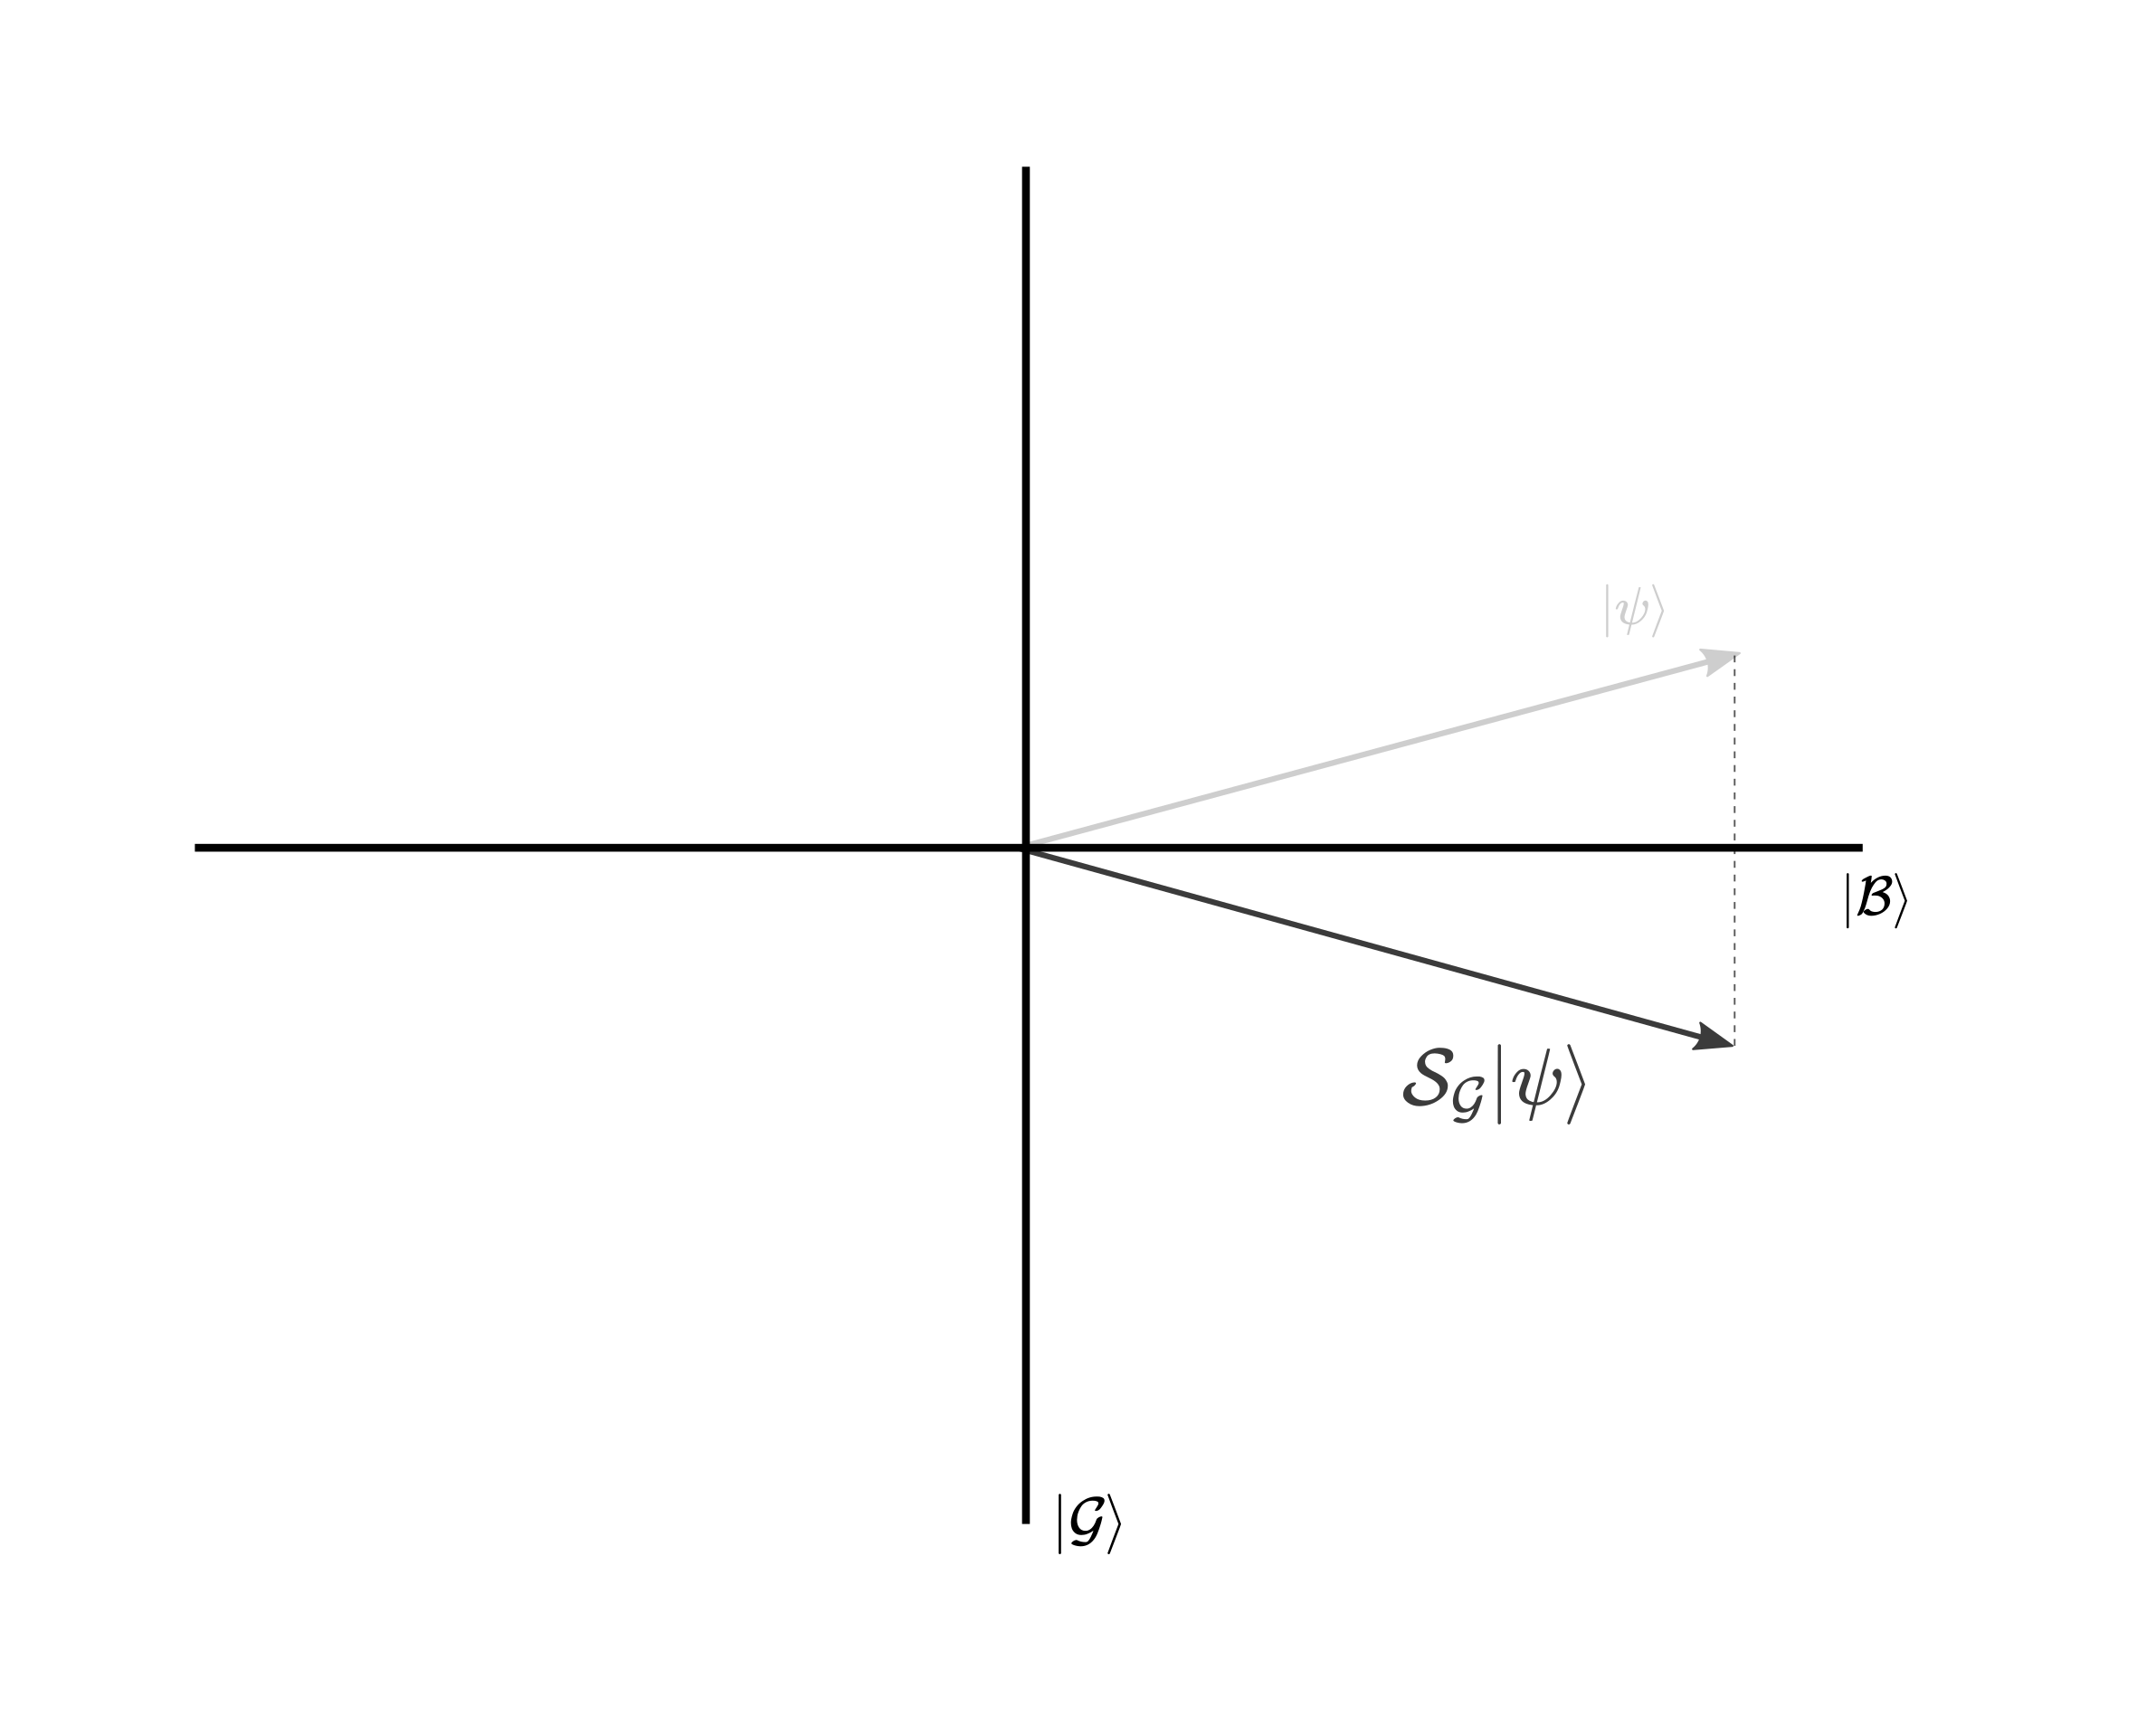
\includegraphics[scale=.87]{psi3.png}
    \end{overprint}
\end{figure}


\end{frame}

%------------------------------------------------


%------------------------------------------------

\begin{frame}{Amplitude Amplification: Visualization II}

    Then apply the operator $ \mathcal{S}_{\mathcal{\psi }} $,

   \begin{figure}
    \begin{overprint}
        \onslide<1>\centering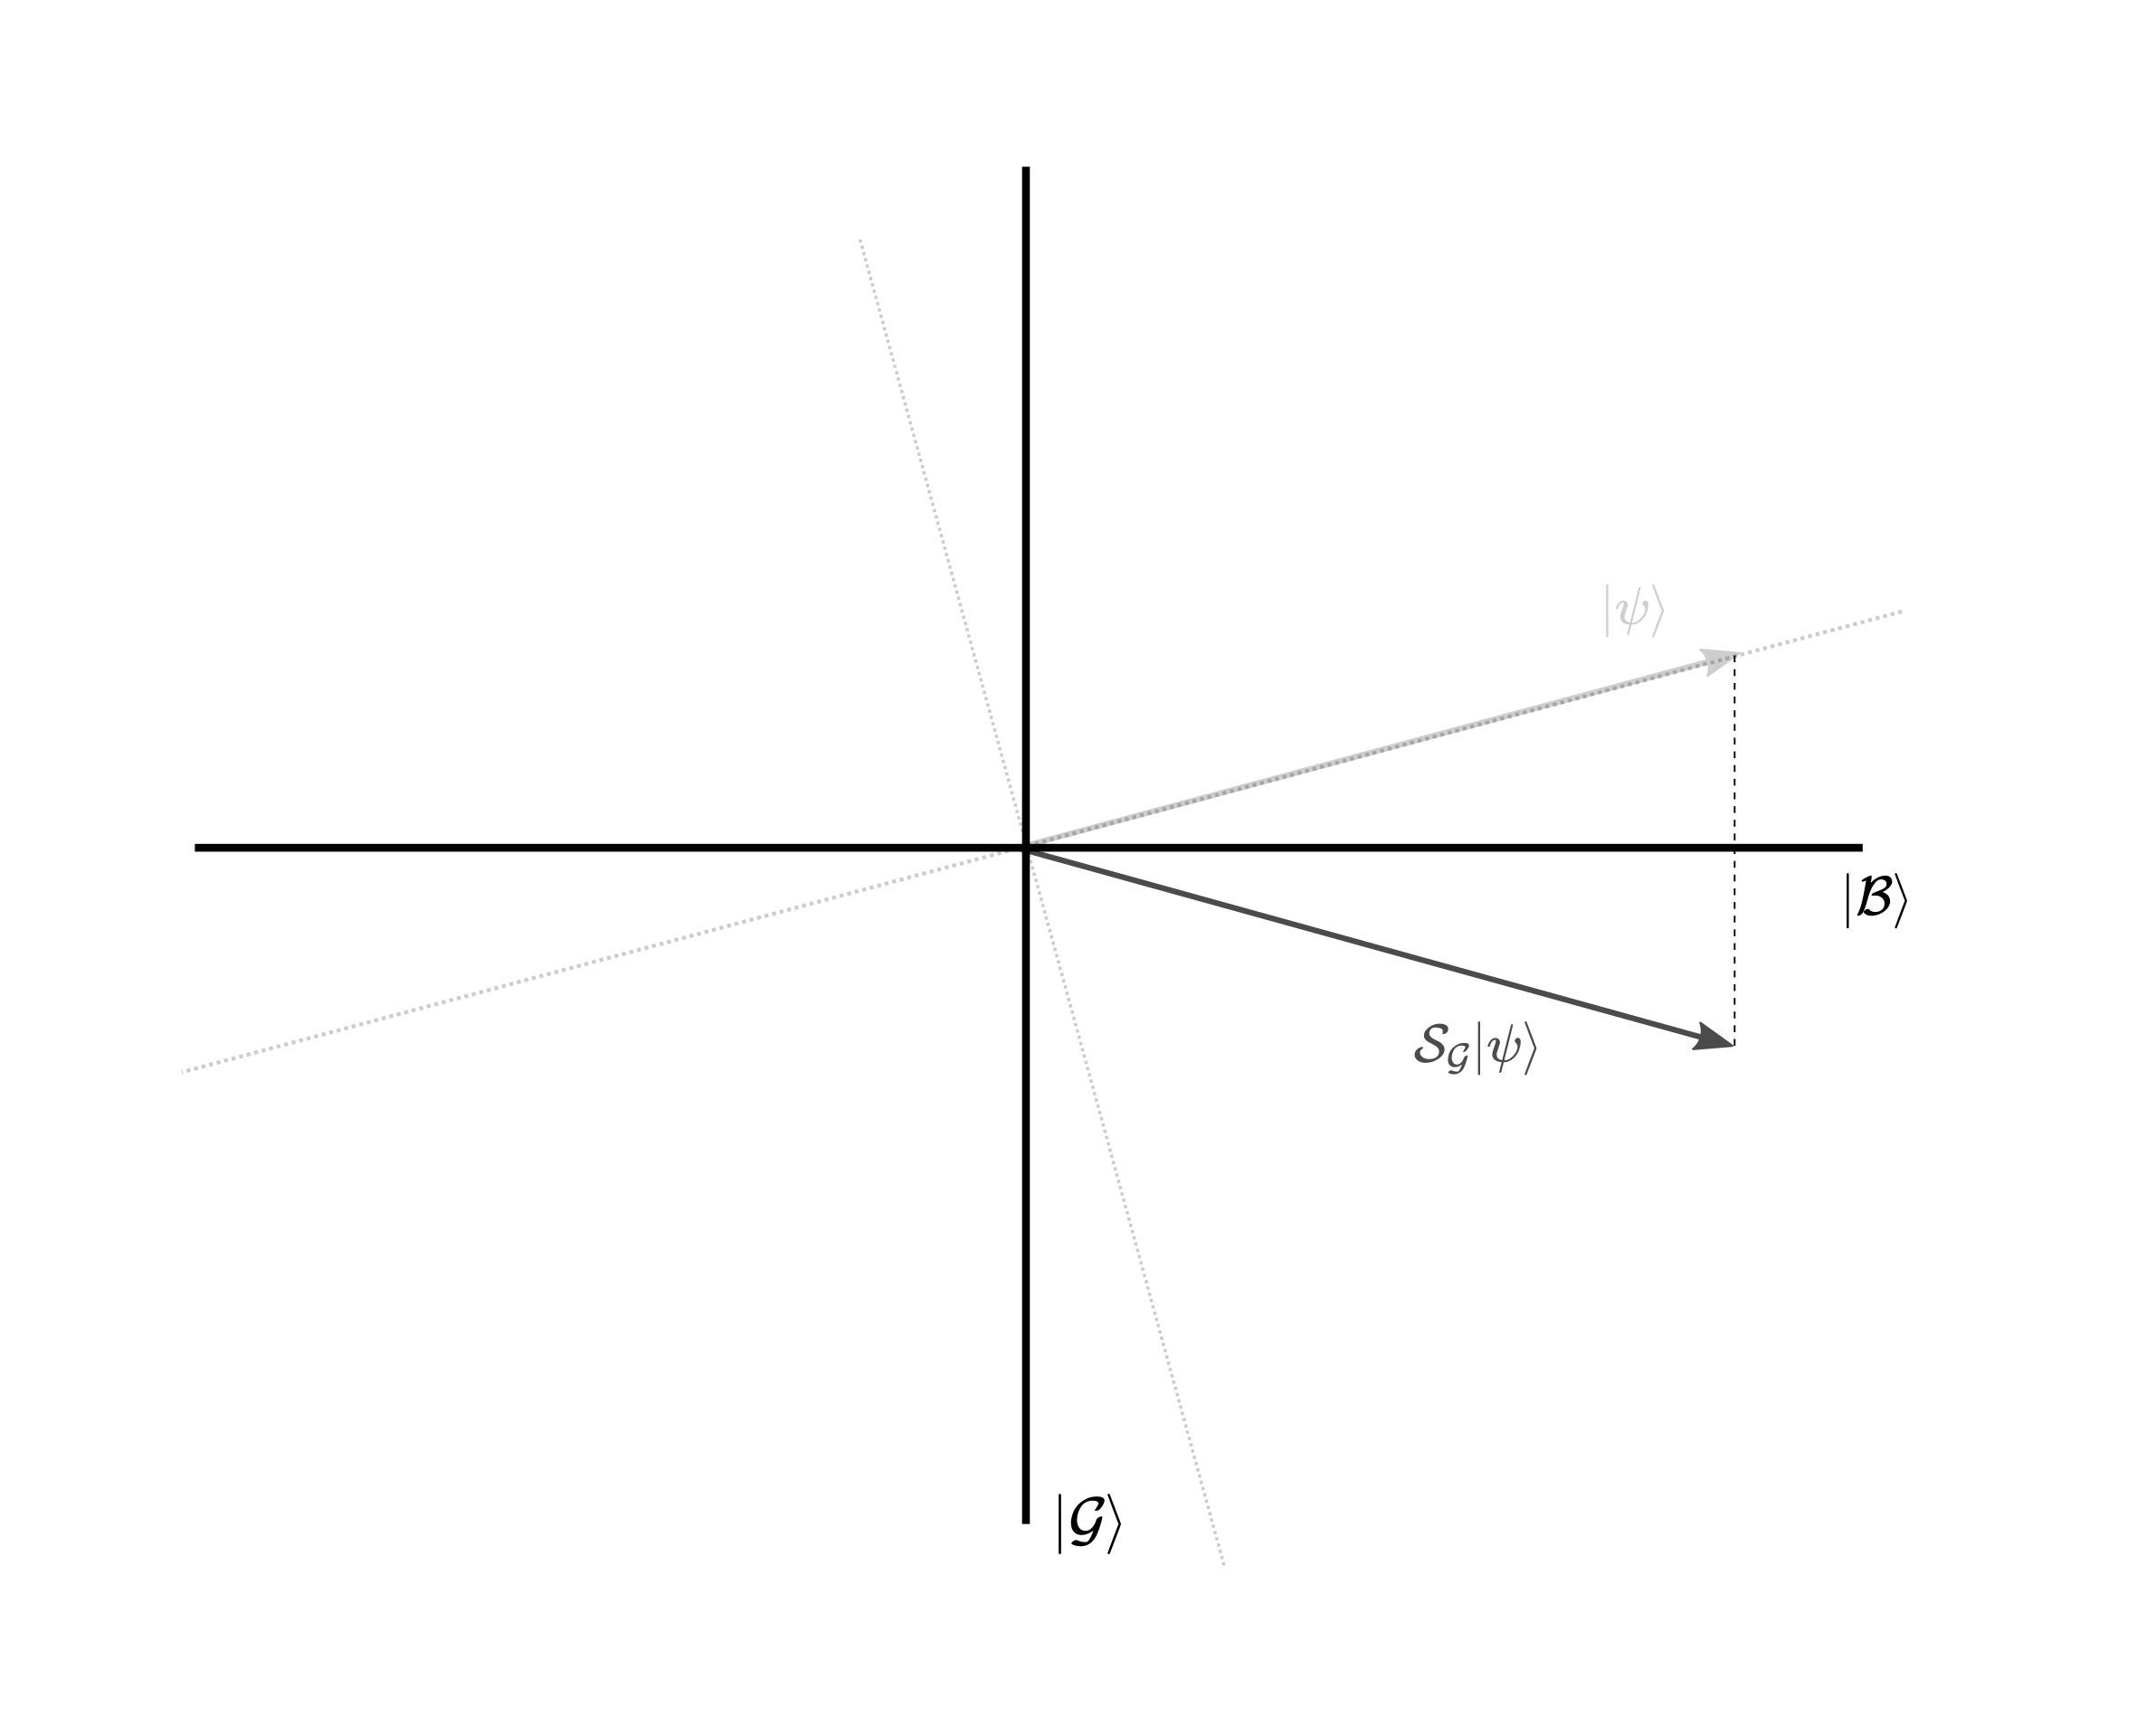
\includegraphics[scale=.87]{psi2_5.png}
        \onslide<2>\centering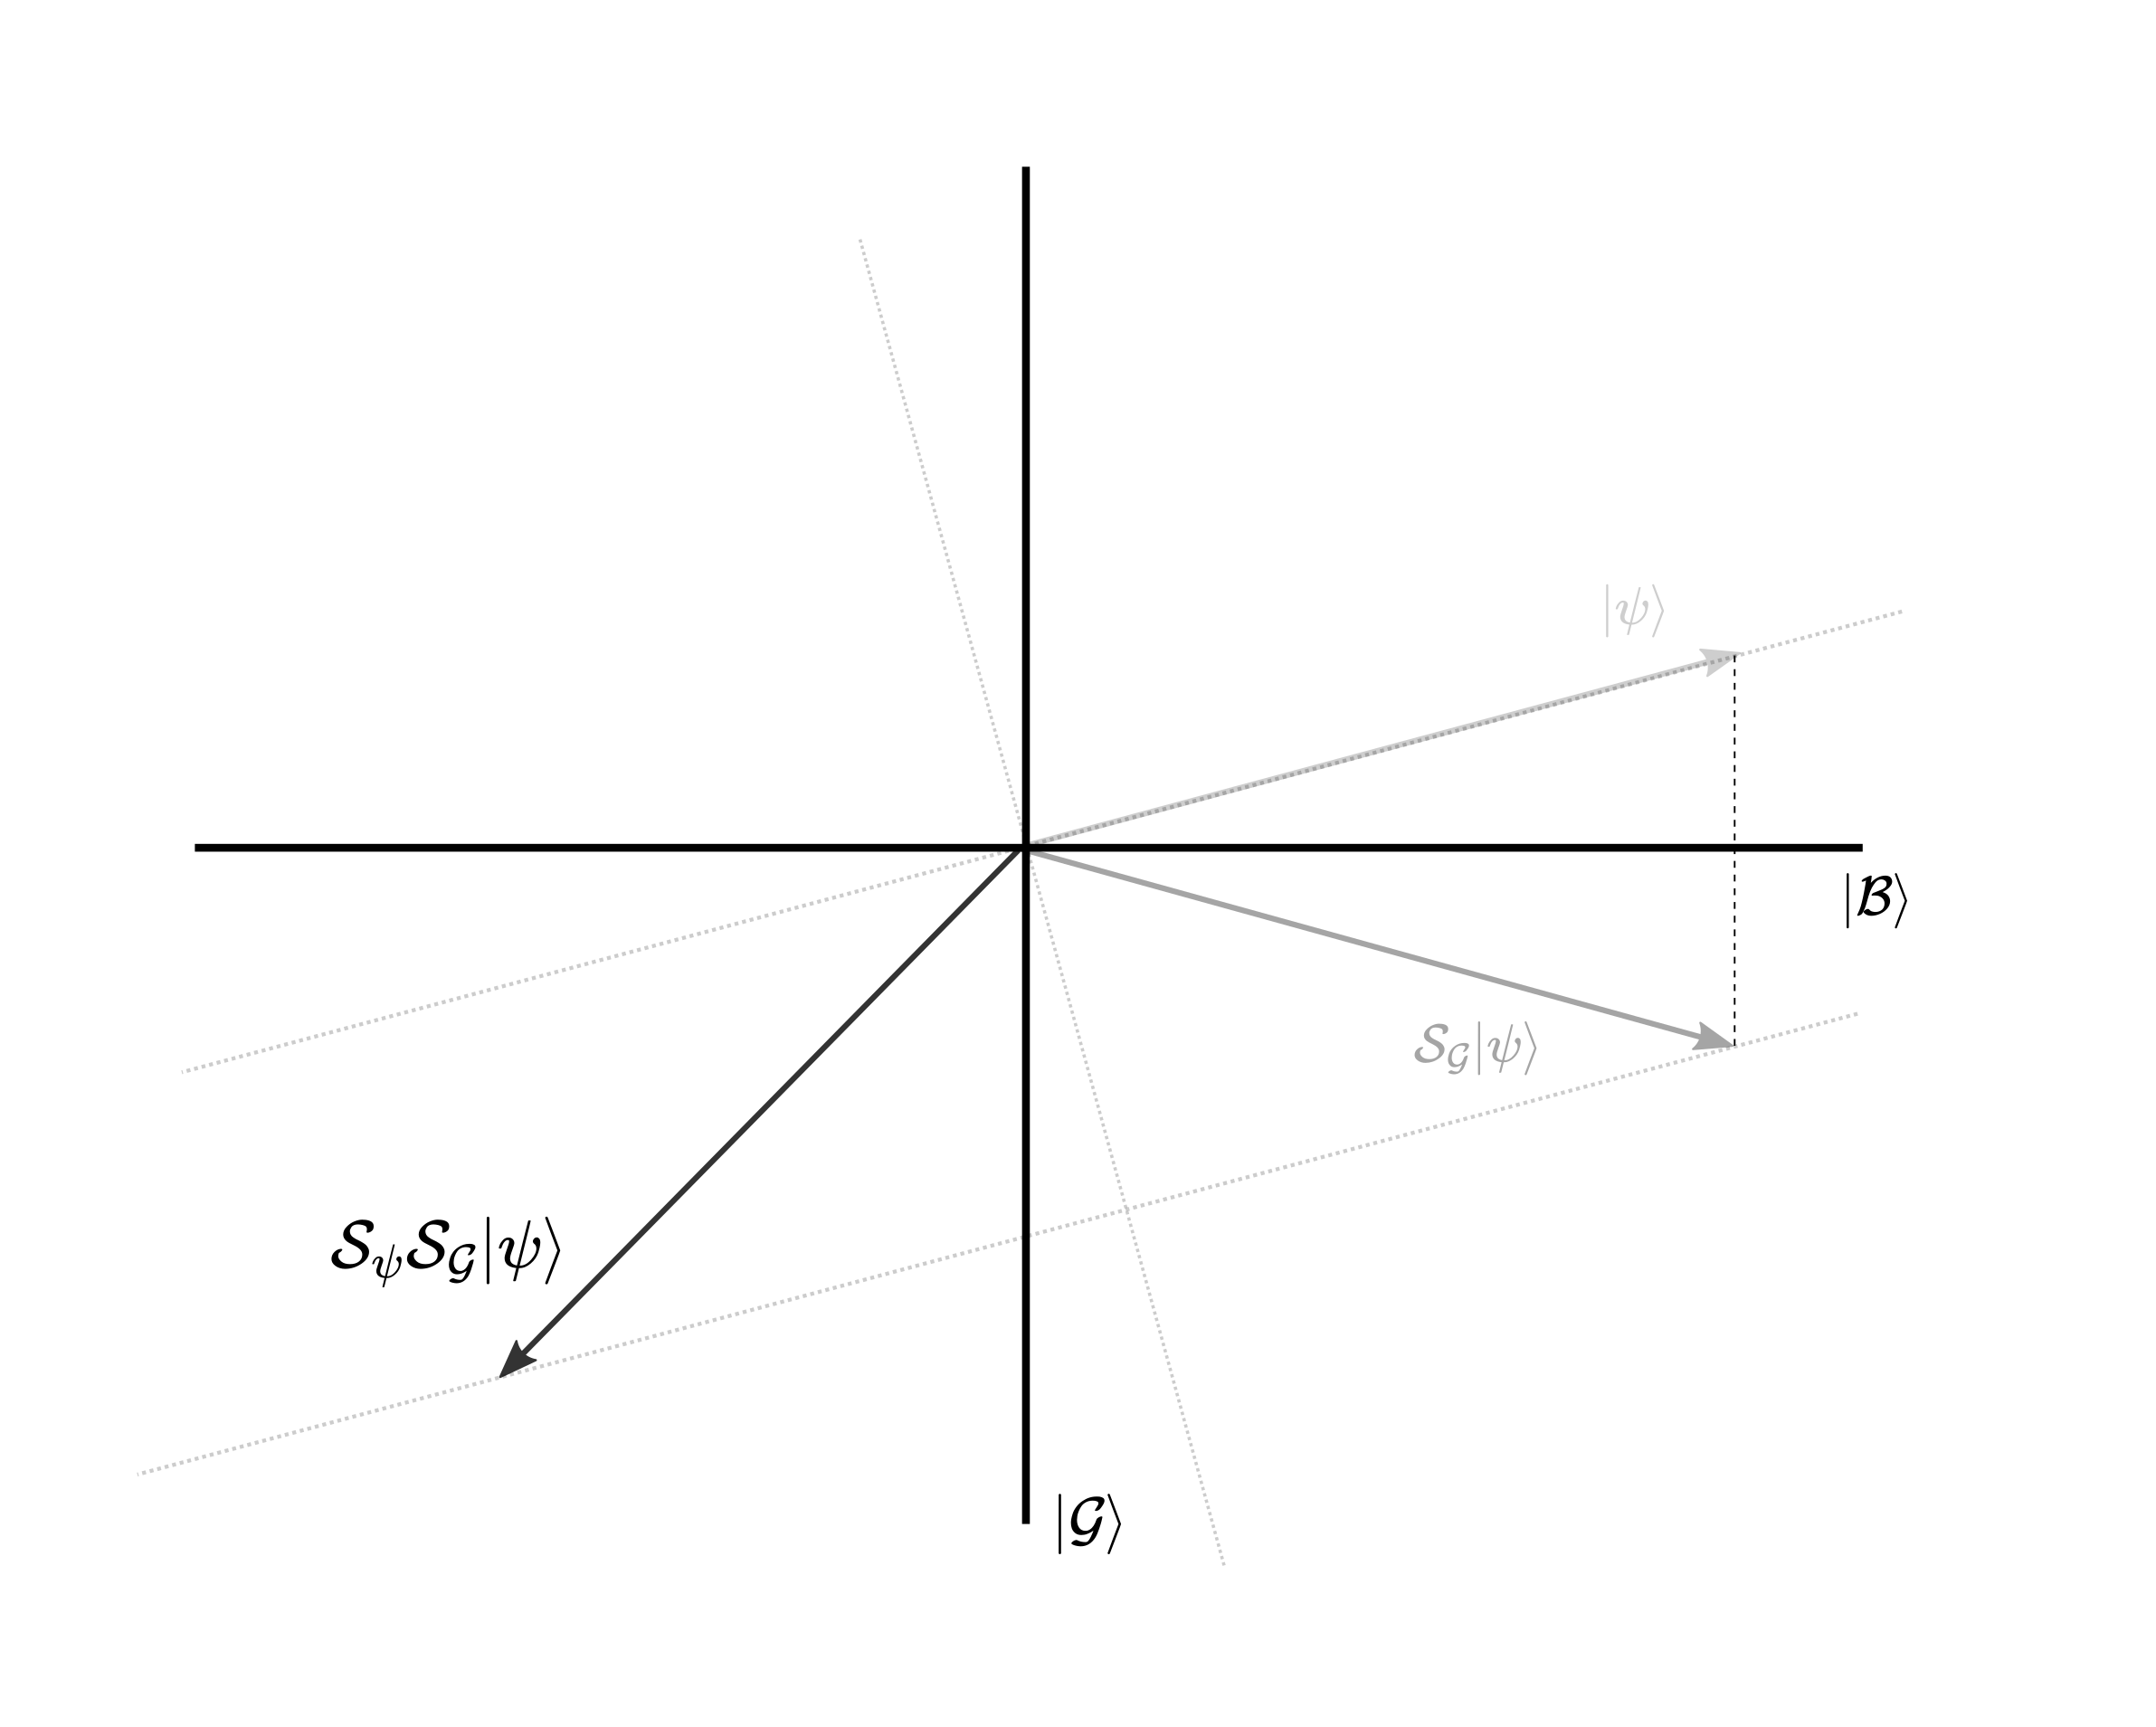
\includegraphics[scale=.87]{psi2.png}
    \end{overprint}
\end{figure}


\end{frame}

%------------------------------------------------

%------------------------------------------------

\begin{frame}{Amplitude Amplification: Visualization III}

    Now, negate the resulting statevector

   \begin{figure}
    \begin{overprint}
        \onslide<1>\centering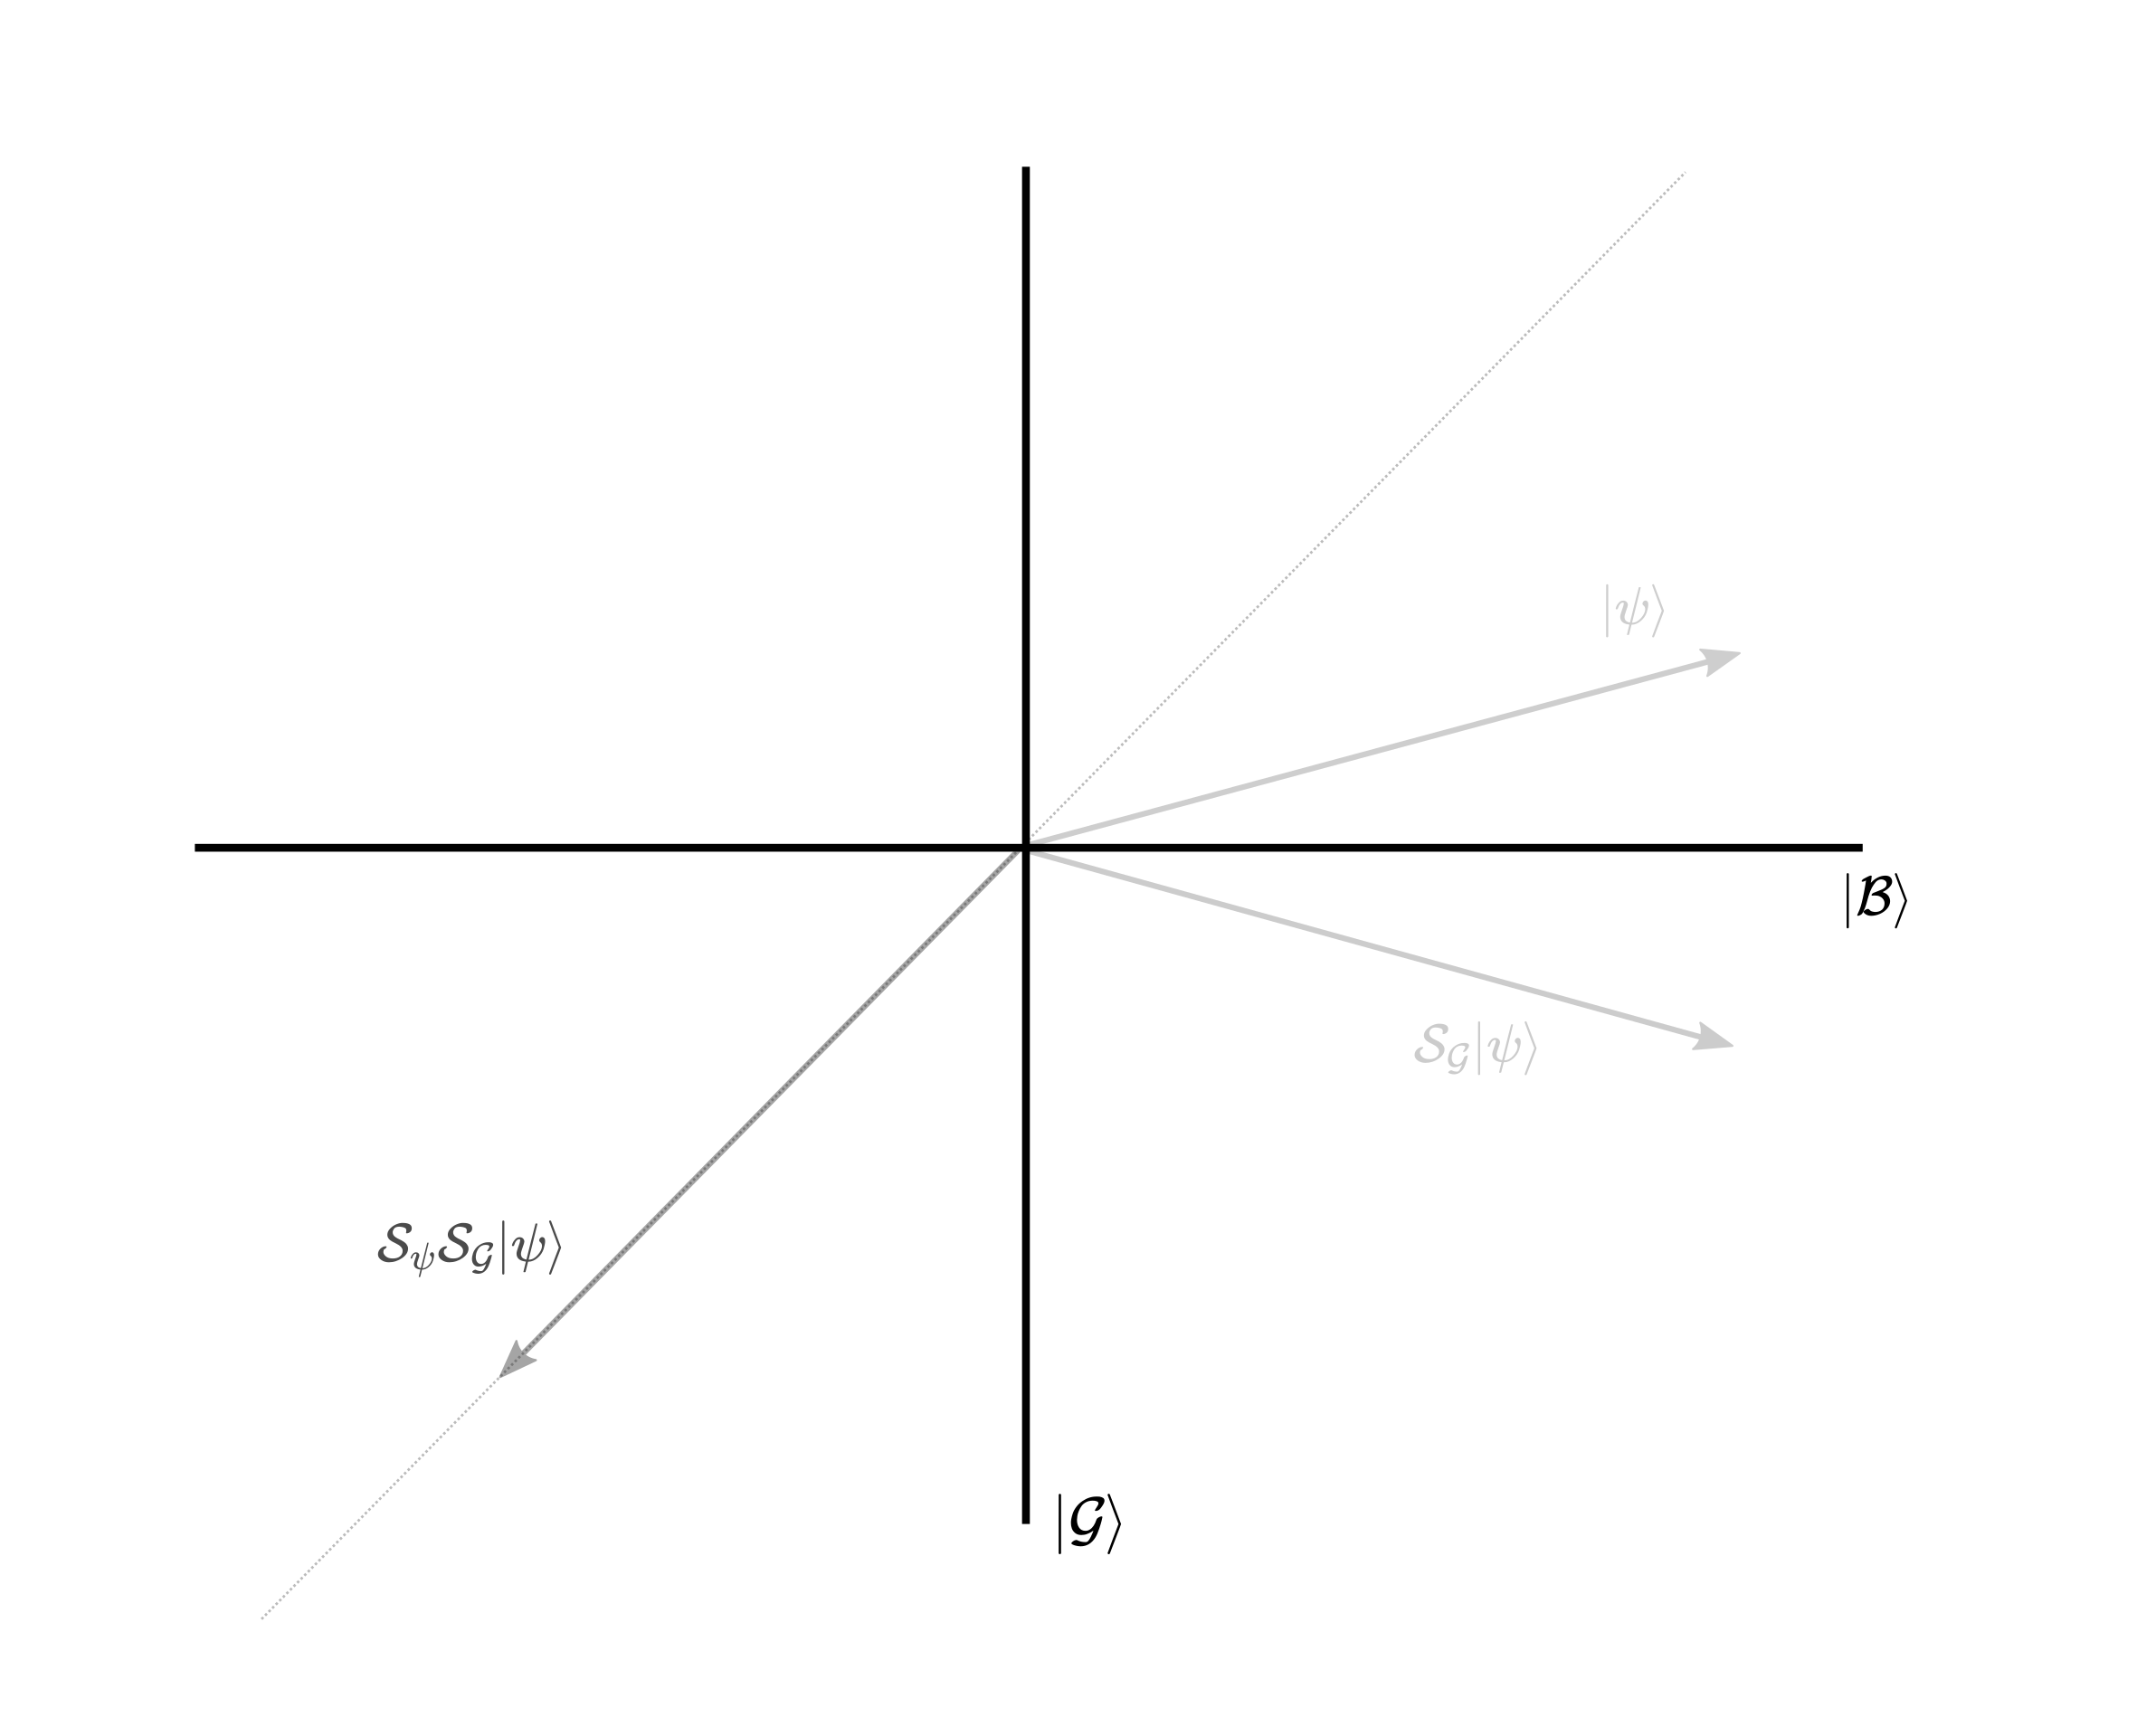
\includegraphics[scale=.87]{psi1_5.png}
        \onslide<2>\centering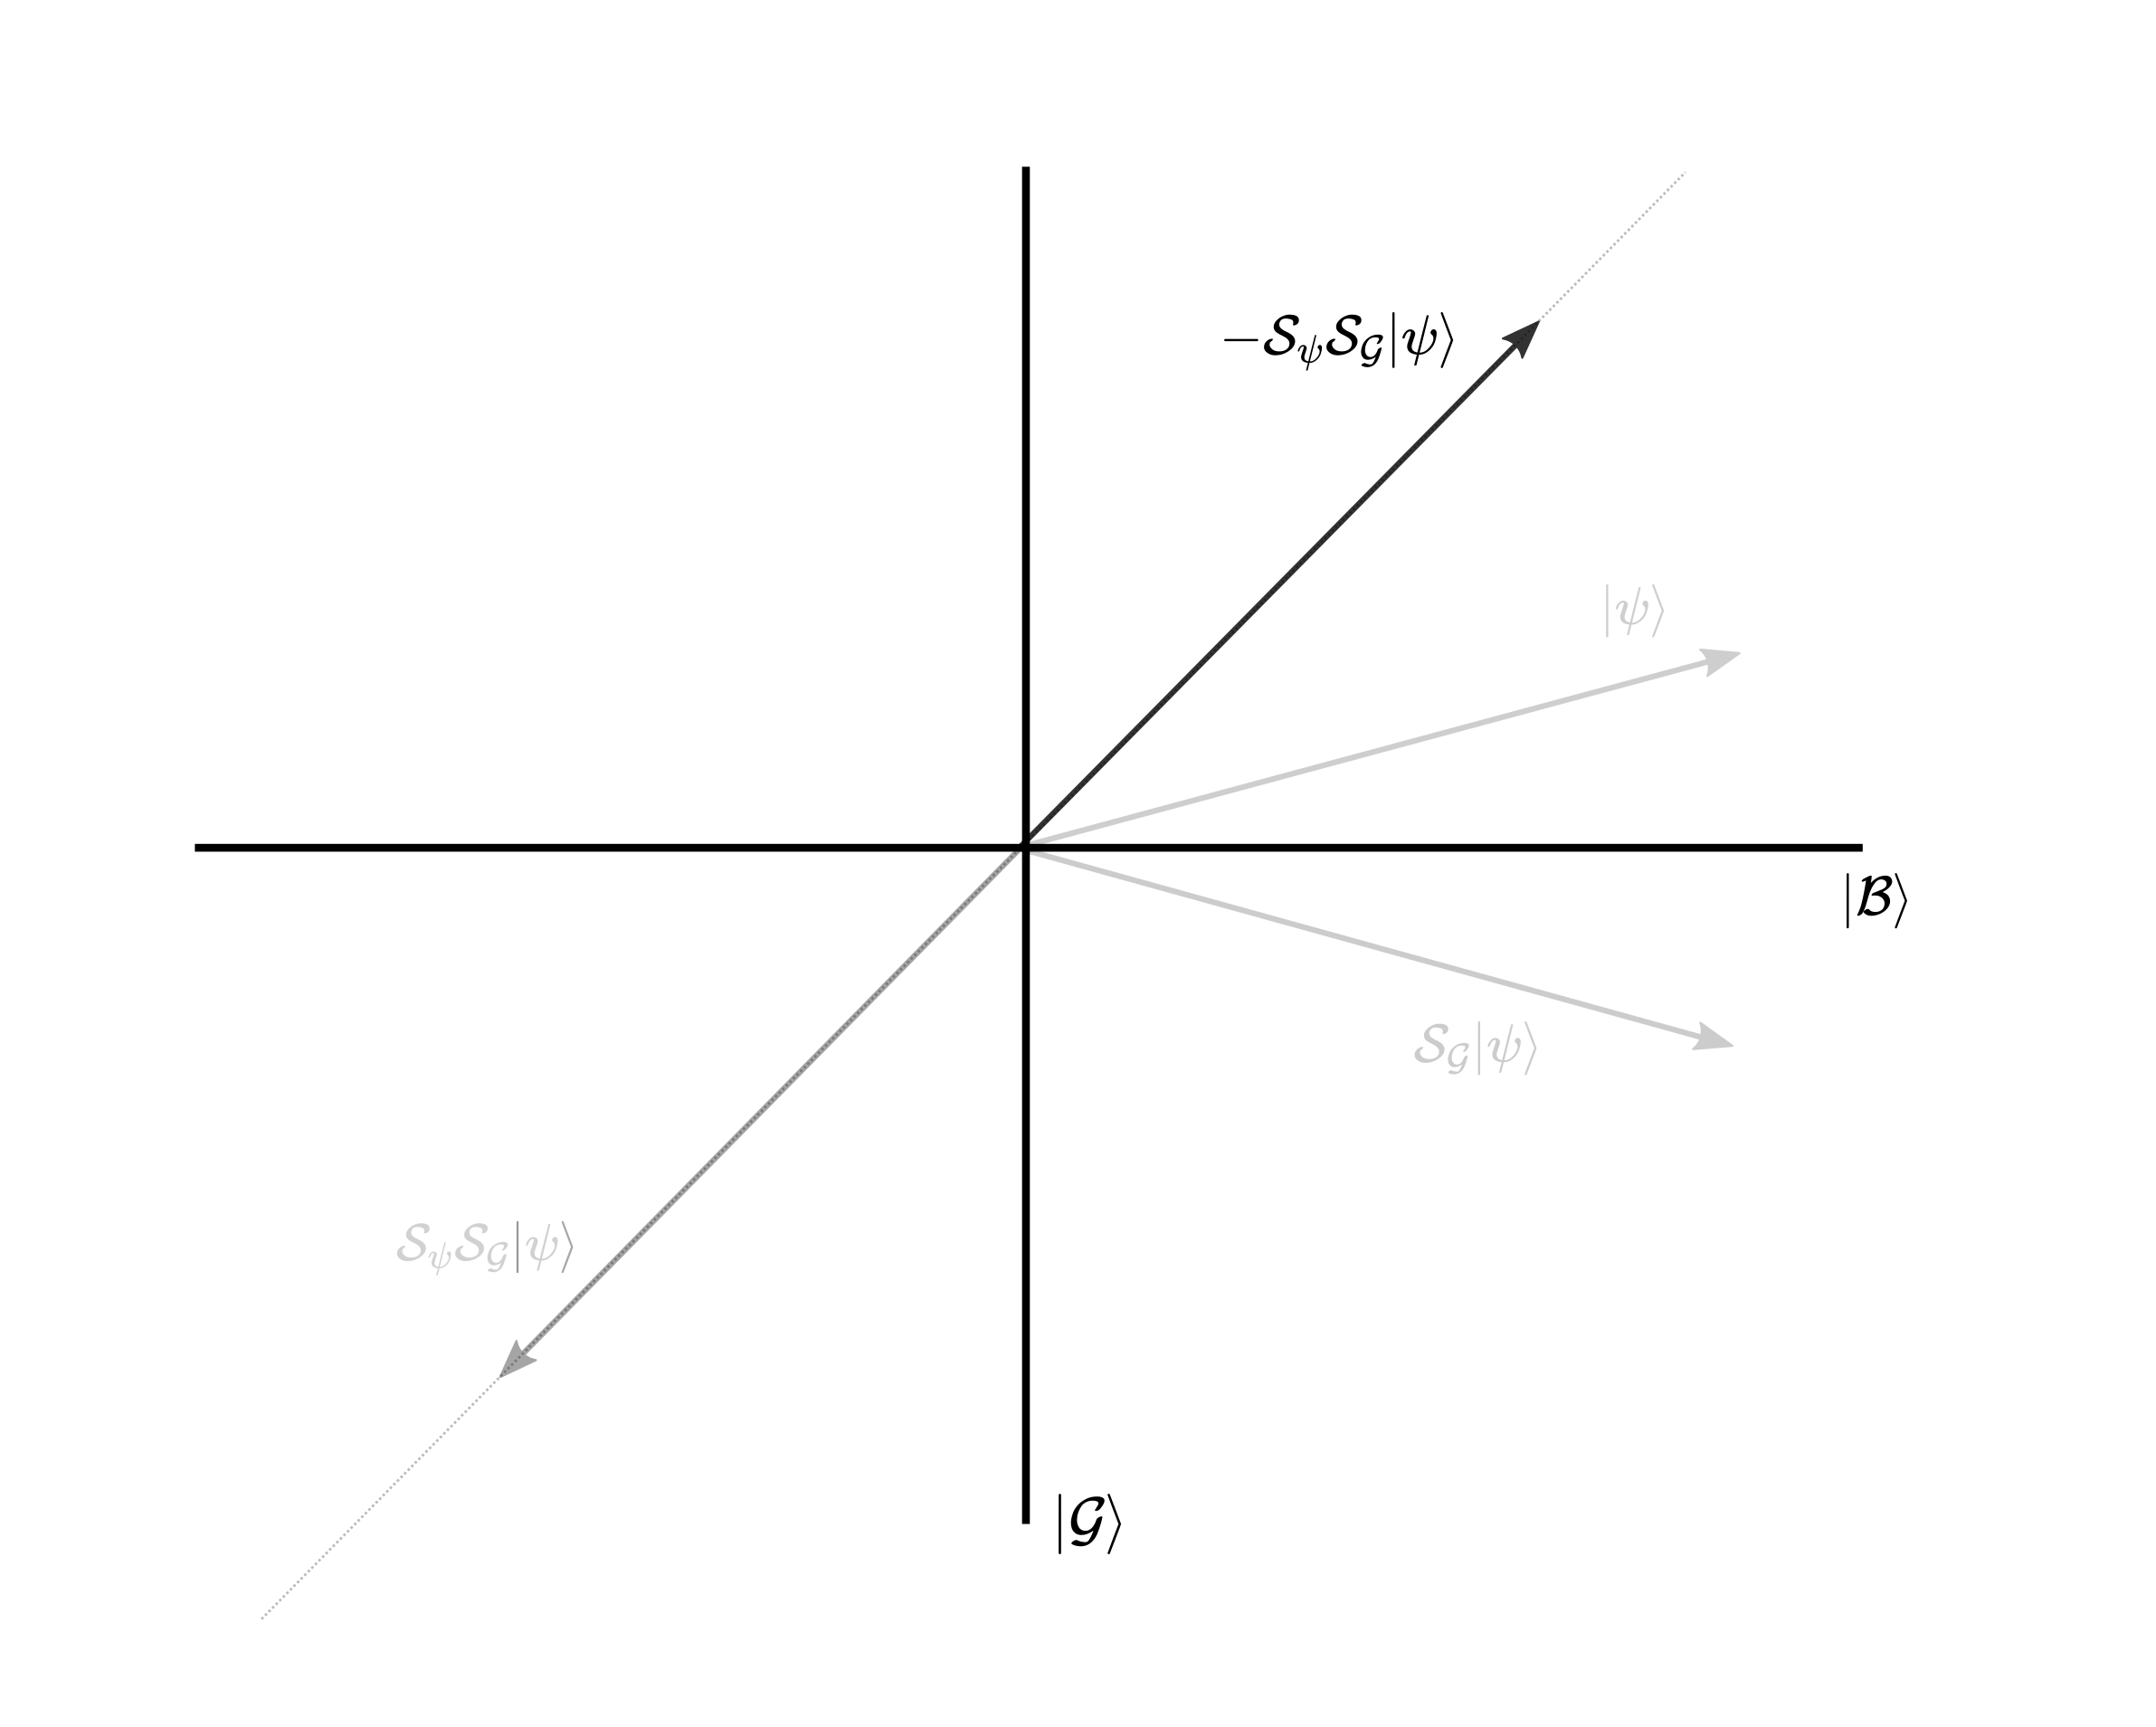
\includegraphics[scale=.87]{psi1.png}
    \end{overprint}
\end{figure}


\end{frame}

%------------------------------------------------

%------------------------------------------------

\begin{frame}{Amplitude Amplification: Visualization IV}

    \hspace{-.5cm }And voil\'a! 

    \vspace{-.2cm}

        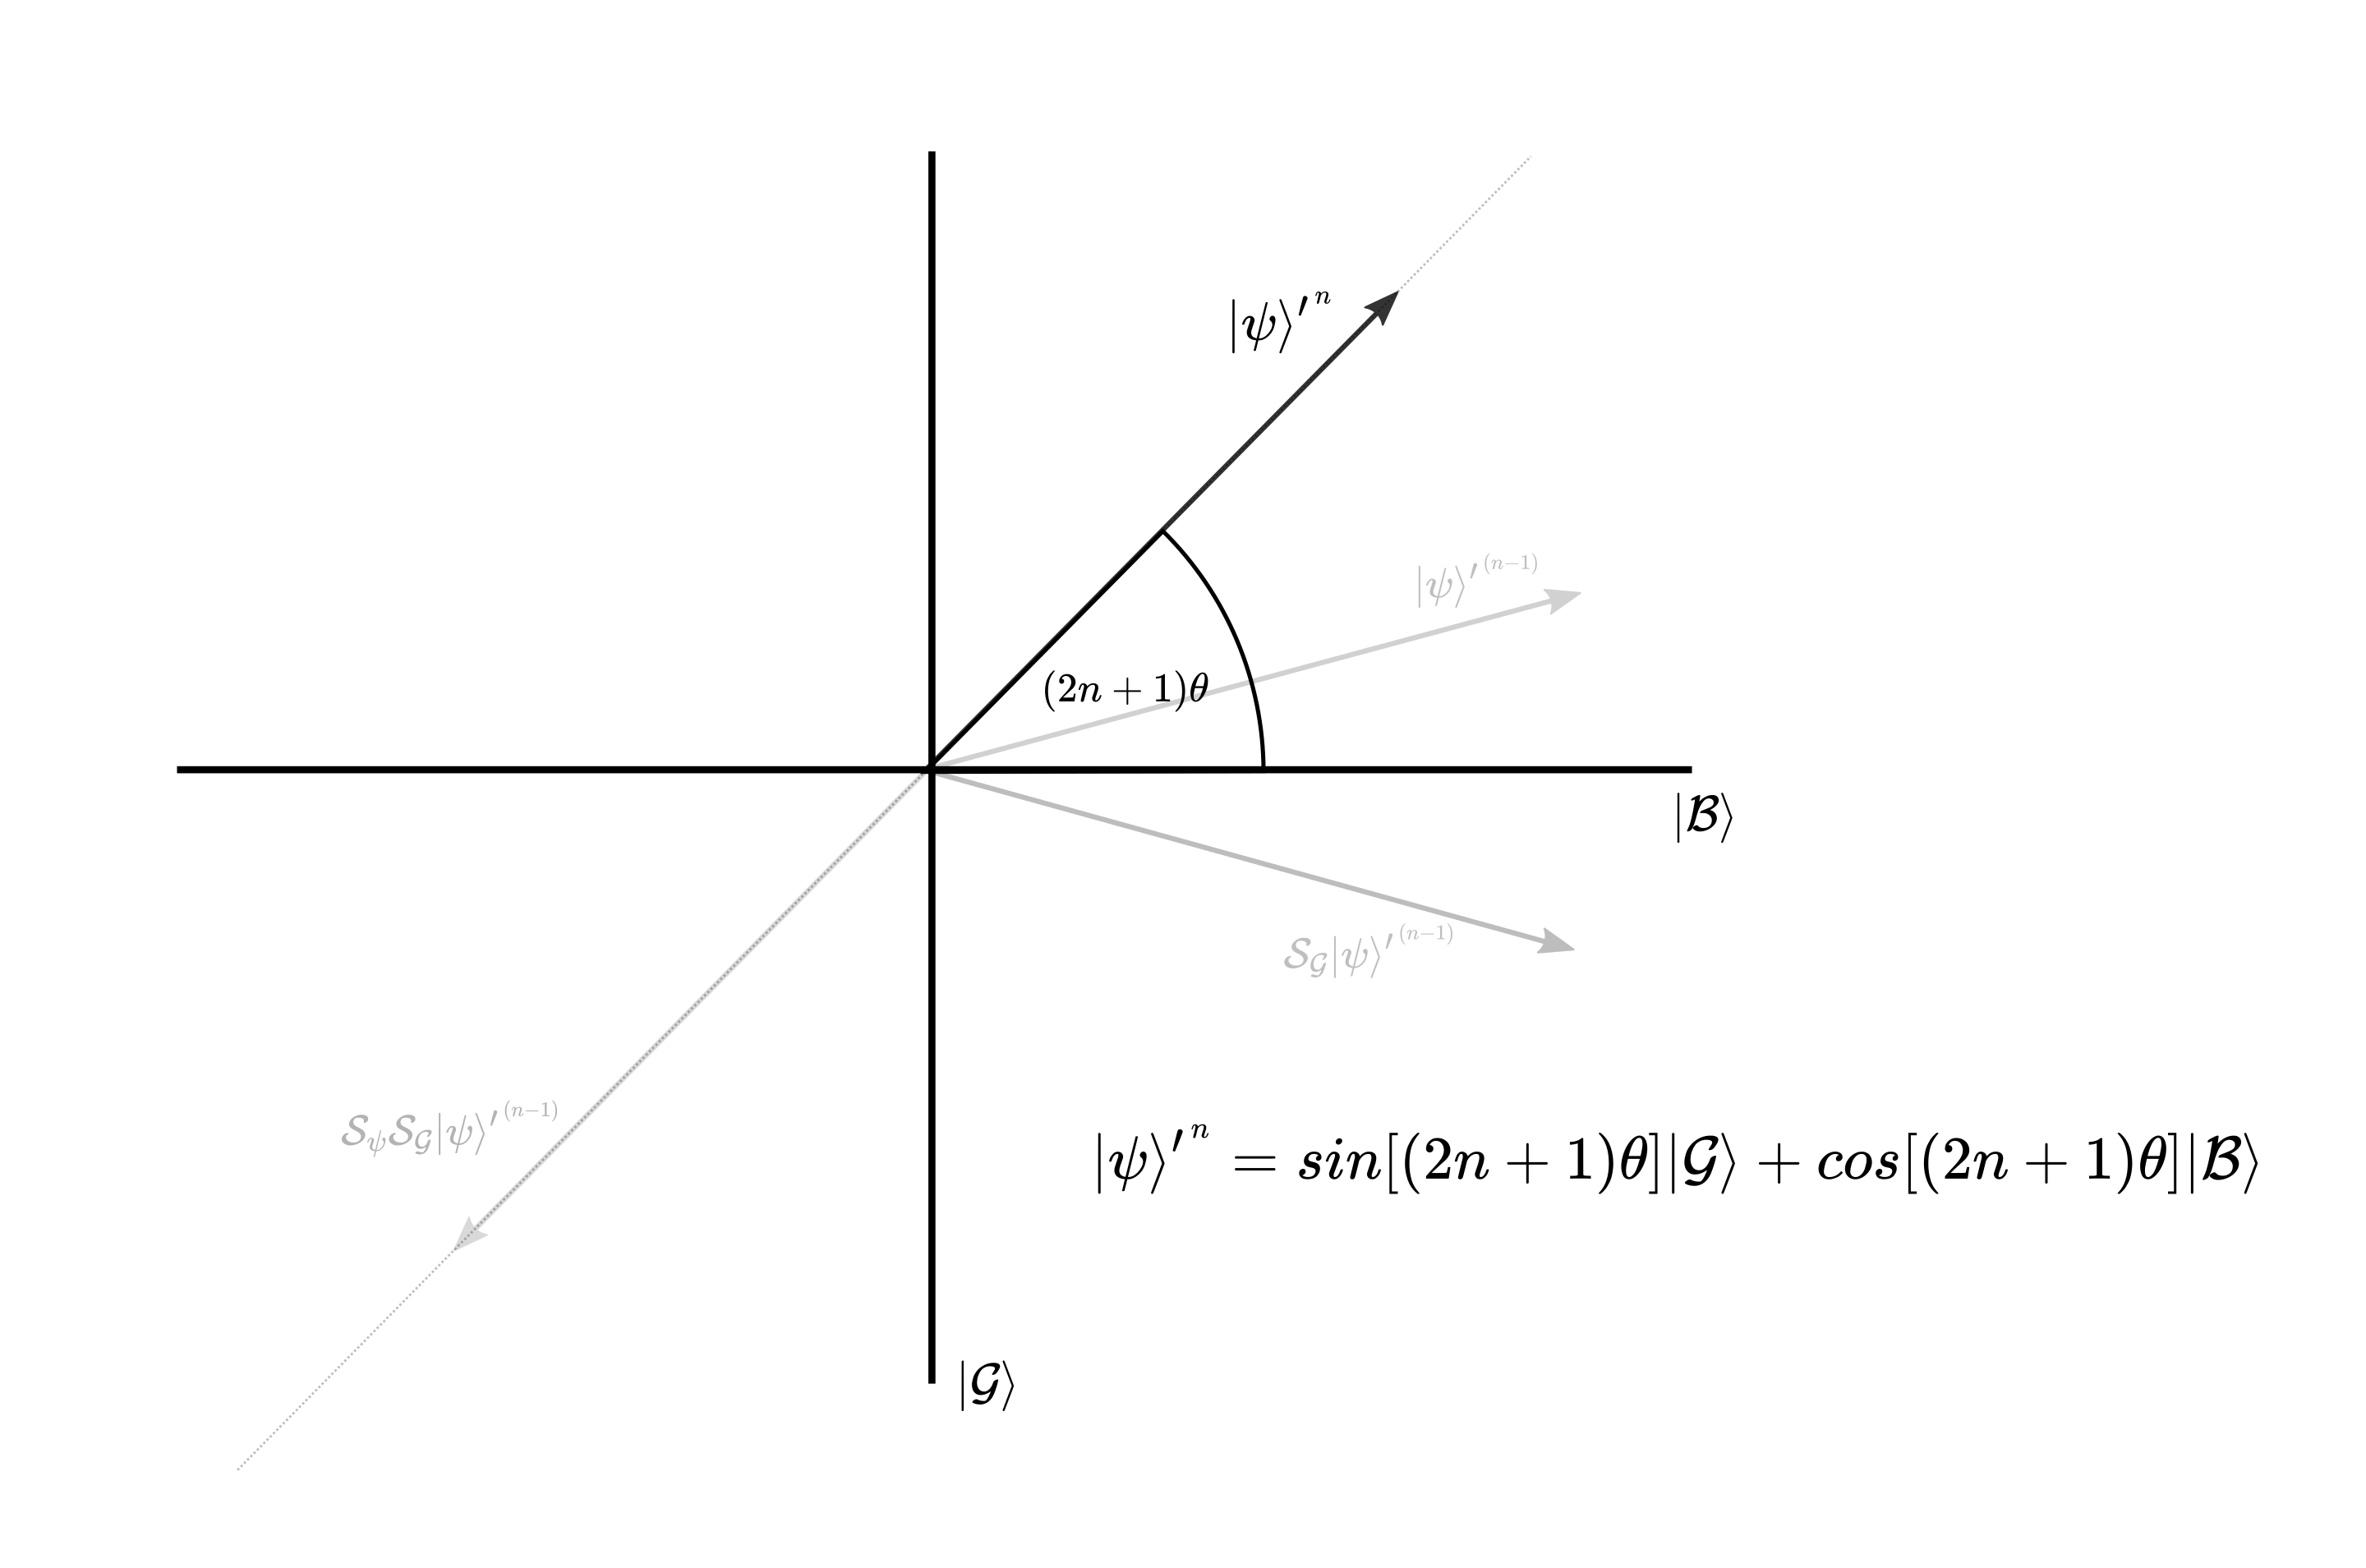
\includegraphics[scale=.87]{psifin.png}
        \pause

\vspace{-.45cm}

\hspace{1.3cm}Though, we'd need to know $n$ as well\pause. Ideally $\lfloor \frac{\pi}{4\theta }  \rfloor$\pause

Now, let's do some coding!


\end{frame}

%------------------------------------------------



%------------------------------------------------
\begin{frame}{Qiskit}
	\begin{columns}[c] % The "c" option specifies centered vertical alignment while the "t" option is used for top vertical alignment
		

		
		\column{.5\textwidth} % Right column and width
	    Qiskit is a quantum software devlopment kit with a python front-end partially
        developed by IBM.\pause

		\column{.45\textwidth} % Left column and width
		\textbf{Features}
		\begin{enumerate}
			\item Simulate + visualize quantum circuits you create 
                yourself\pause
			\item Compatible with IBM's current quantum computers\pause
			\item Vibrant and active online community
		\end{enumerate}
	\end{columns}
\end{frame}

%------------------------------------------------


%------------------------------------------------

\begin{frame}{Running the QFT}
    Let's run the QFT on some states in Qiskit. \pause We'll use a statevector simulation. \pause 
    The local evolution of the qubits is depicted in the bloch spheres below:

    \medskip\pause

\hspace{-1.2cm}
\begin{minipage}[c]{0.25\textwidth}
    Input: $\vert 000 \rangle \rightarrow$
\end{minipage}
\begin{minipage}[c]{0.33\textwidth}
    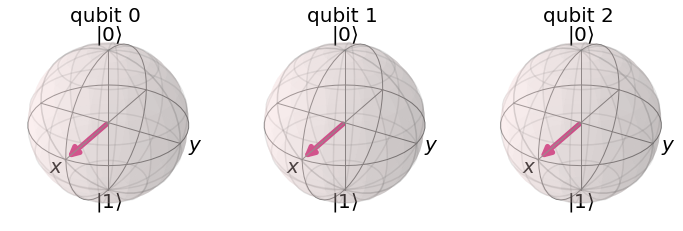
\includegraphics[scale=.2]{q000.png}
\end{minipage}

    \medskip\pause

\hspace{-1.2cm}
\begin{minipage}[c]{0.25\textwidth}
    Input: $\vert 001 \rangle \rightarrow$
\end{minipage}
\begin{minipage}[c]{0.33\textwidth}
    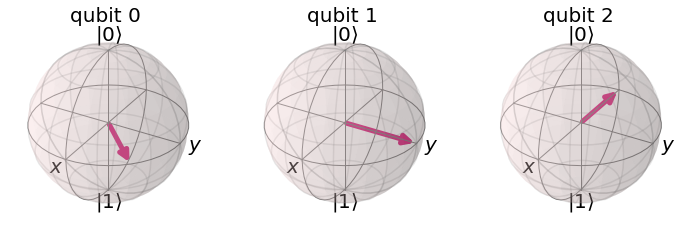
\includegraphics[scale=.2]{q001.png}
\end{minipage}

    \medskip\pause

\hspace{-1.2cm}
\begin{minipage}[c]{0.25\textwidth}
    Input: $\vert 010 \rangle \rightarrow$
\end{minipage}
\begin{minipage}[c]{0.33\textwidth}
    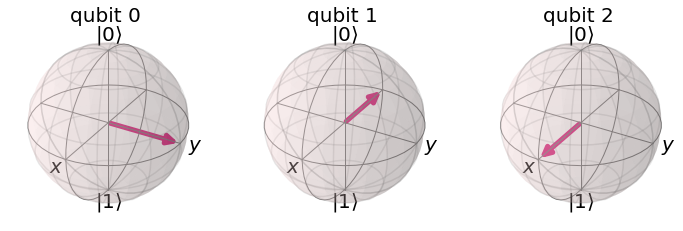
\includegraphics[scale=.2]{q010.png}
\end{minipage}



\end{frame}


%------------------------------------------------




%------------------------------------------------

\begin{frame}[fragile]{Where's the code?}

    For the QFT transforms just shown, it's rather simple:\pause

    \vspace{.4cm}

\begin{pyverbatim}
from qiskit.circuit.library import QFT
qft = QFT(3)
qft3_000 = execute(qft, backend).result()
plot_bloch_multivector(qft3_000.get_statevector())
\end{pyverbatim}

    \vspace{.4cm}\pause

    Moving forward, I'll just link the code online.

\end{frame}


%------------------------------------------------




%------------------------------------------------

\begin{frame}{Finding Phases}
    Let's run the 3-qubit phase estimation algorithim on some gates.\pause

    \medskip

    We'll use controlled phase gates\pause, with matrices of the form

    \medskip

    $$ CP\left(  \alpha   \right)= 
    \begin{bmatrix}
        1 & 0 & 0 & 0 \\
        0 & 1 & 0 & 0 \\
        0 & 0 & 1 & 0 \\
        0 & 0 & 0 & e^{i\alpha }\\ 
    \end{bmatrix}.
    $$\pause
    
     We already know that $\vert 1 \rangle $ is an
     eigenvector of basic phase gates.
\end{frame}


%------------------------------------------------

%------------------------------------------------

\begin{frame}{Finding Phases: CP($\pi /4$)}
    This time, we'll use the qasm simulator\pause. This lets us get counts of
    simulated measurements at the end\pause. So, let's see the circuit:\pause

    \medskip

    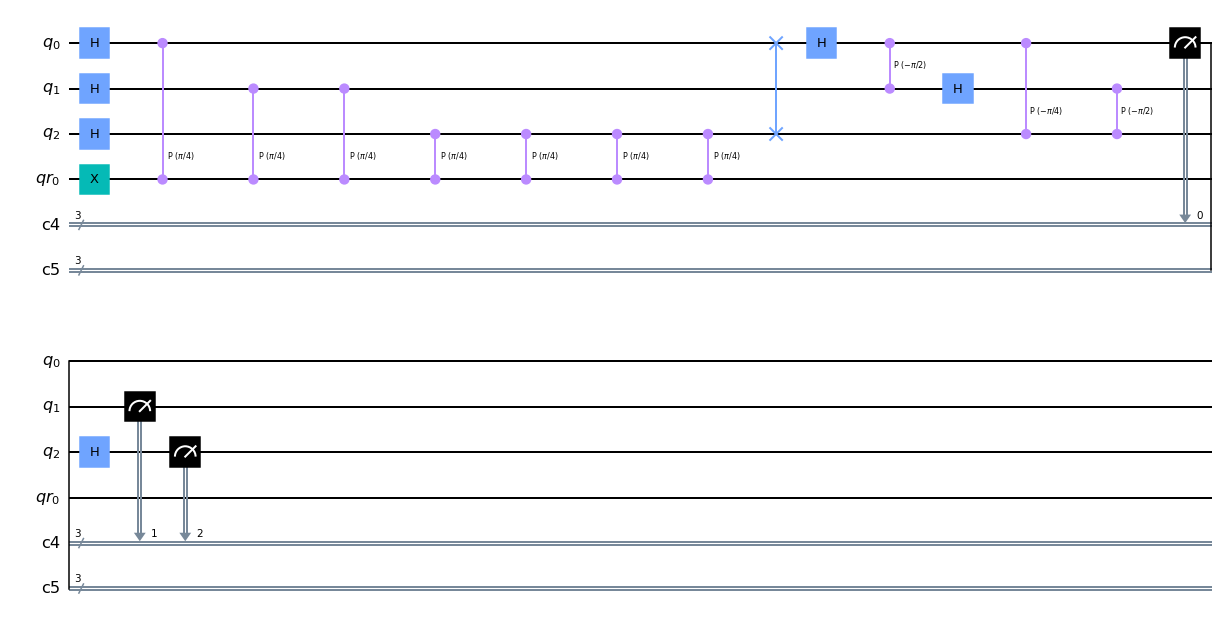
\includegraphics[scale=.23]{cppi4.png}
\end{frame}


%------------------------------------------------

%------------------------------------------------

\begin{frame}{Finding Phases: CP($\pi /4$)}
    Running the simulation gives a simulated measurement set:\pause

    \medskip

    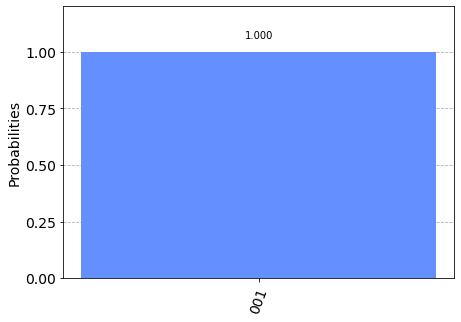
\includegraphics[scale=.45]{pepi4counts.png}\pause

    \vspace{.4cm}

    Is this what we would expect? \pause Yes! \pause

   As the phase can be encoded perfectly
   in 3 qubits, we should expect
    the output vector to be $\vert k \rangle =$
       $\vert \alpha  \frac{2^{n-1} }{\pi }\rangle $ \pause or
       $ \vert 001 \rangle $ in binary

\end{frame}


%------------------------------------------------


%------------------------------------------------

\begin{frame}{Finding Phases: CP($5\pi /4$)}
    Let's try it again with another ideal phase:
    \pause

    \medskip

    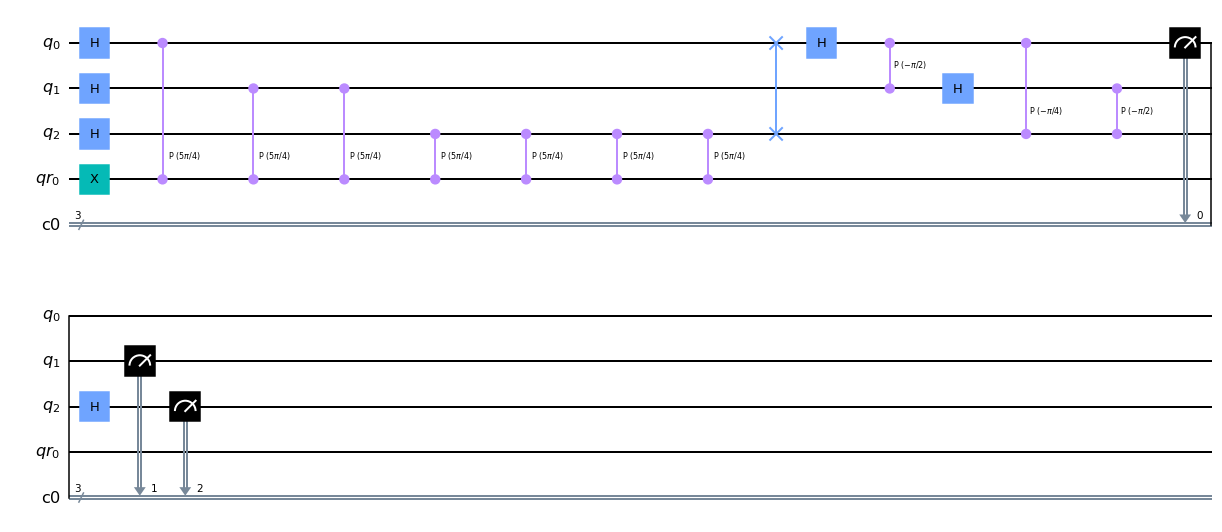
\includegraphics[scale=.23]{cp5pi4.png}

    \vspace{.4cm}


\end{frame}


%------------------------------------------------


%------------------------------------------------

\begin{frame}{Finding Phases: CP($5\pi /4$)}
    
    Now, we should get $\vert 5 \rangle=\vert 101\rangle$:
    \pause

    \medskip

    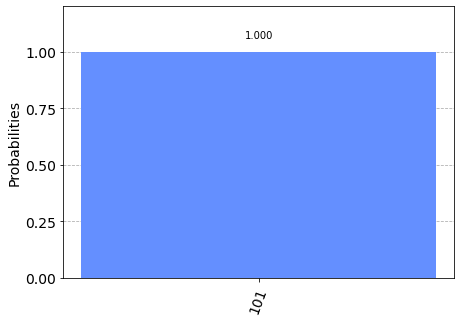
\includegraphics[scale=.45]{pe5pi4counts.png}
    \vspace{.4cm}

    Yup!
\end{frame}


%------------------------------------------------

%------------------------------------------------

\begin{frame}{Finding Phases: CP($4\pi /5$)}
    
    Let's try something that's not an ideal phase:
    \pause

    \medskip

    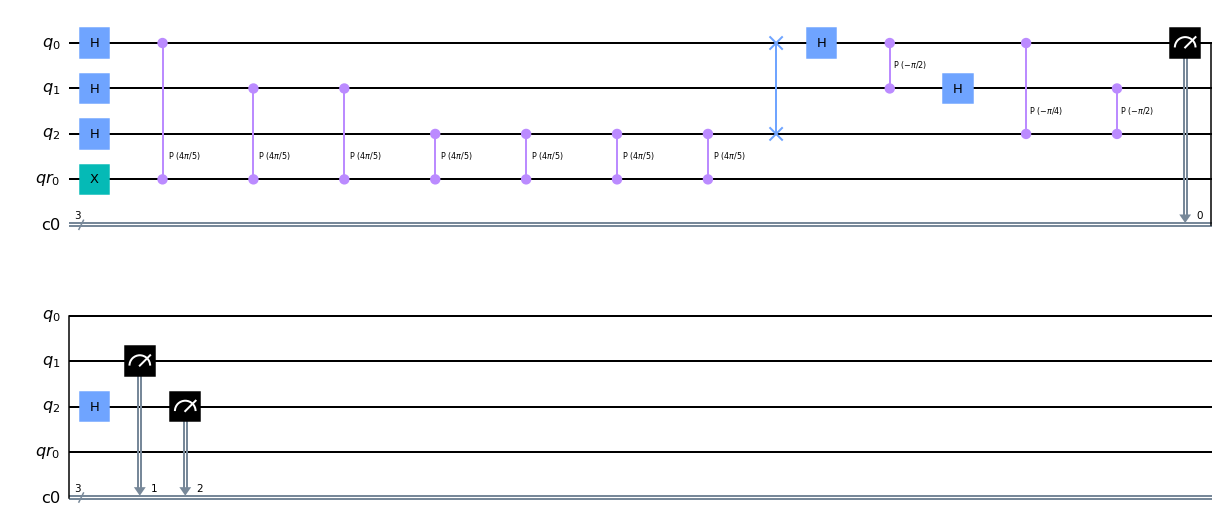
\includegraphics[scale=.23]{cp4pi5.png}
    \vspace{.4cm}

\end{frame}


%------------------------------------------------

%------------------------------------------------

\begin{frame}{Finding Phases: CP($4\pi /5$)}
    
    Let's see what we get when we run the simulation several times:
    \pause

    \medskip

    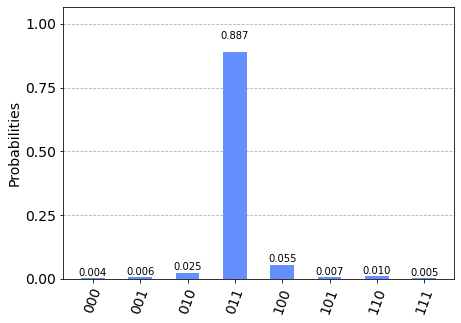
\includegraphics[scale=.45]{pe4pi5counts.png}\pause

    \vspace{.4cm}

     This seems to be a good estimate given $ \frac{4\pi }{5} \frac{4}{\pi } =3.2 \approx 3$.\pause

     \medskip

     Let's do some amplitude amplification!
    
\end{frame}


%------------------------------------------------


%------------------------------------------------

\begin{frame}{Amplitude Amplification in Practice}

    Below is a simple 2-qubit circuit for amplitude amplification that searches for the
    $\vert 11 \rangle $ state:

    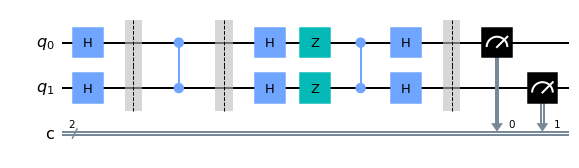
\includegraphics[scale=.5]{grovercirc11.png}

    \pause

    The first section initializes the state into $\vert + \rangle ^{\otimes 2}  $\pause.

    The second 
    portion flips the sign of only $\vert 11 \rangle $\pause. 

    The third section flips
    the state about the original vector.\pause 

    We only need to run the operations once as
    $n=1$ here\pause.

    \vspace{.43cm}

    Let's run it!
 
\end{frame}

%------------------------------------------------

%------------------------------------------------

\begin{frame}{Amplitude Amplification in Practice: Simulation}
   
    Running the previous circuit on the simulation we used for phase estimation:

    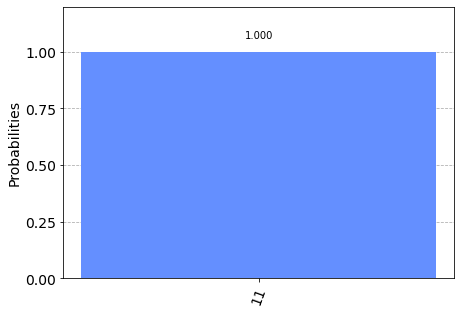
\includegraphics[scale=.45]{groversim.png}

    \vspace{.43cm}\pause

    Perfect results! \pause \ Let's run it for real!
 
\end{frame}

%------------------------------------------------

%------------------------------------------------

\begin{frame}{Amplitude Amplification in Practice: Calling IBMQ}
   
    Now, running our circuit on IBMQ-Lima, a real 5-qubit quantum computer:\pause

    \medskip

    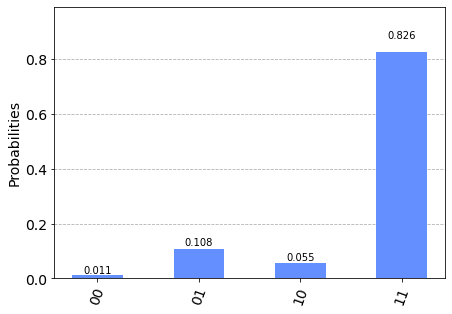
\includegraphics[scale=.45]{groverreal.png}

    \vspace{.43cm}\pause

    Not too bad! 
\end{frame}

%------------------------------------------------

%------------------------------------------------

\begin{frame}{Wrapping Up!}
 
    Basic Quantum Algorithms\pause
    \begin{itemize}
        \item Quantum Fourier Transform \pause
        \item Phase Estimation\pause
        \item Amplitude Amplification\pause
    \end{itemize}

    \medskip

    \medskip
    
    Qiskit\pause
    \begin{itemize}
        \item Visualize qubit evolution\pause
        \item Simulate experiments on circuits\pause
        \item Run circuits on real computers!
    \end{itemize}

    \medskip

    \medskip
\end{frame}

%------------------------------------------------



%------------------------------------------------

\begin{frame}{Moving Forward}
    
    Where to go from here?\pause

    \begin{itemize}
        \item Build to more complex applications\pause
        \item Extend to quantum machine learning\pause
        \item Run some interesting experiments
    \end{itemize}

\end{frame}

%------------------------------------------------


%------------------------------------------------

\begin{frame}{That's it!}
   
    Notebooks for the circuits run here can be found at \url{https://alexheilman.com}


\end{frame}

%------------------------------------------------






%------------------------------------------------

\begin{frame}[allowframebreaks]{References}
    % This might take more than one page
    \nocite{*}
    \printbibliography

\end{frame}

%------------------------------------------------

\begin{frame}
    \Huge{\centerline{Thanks}}
\end{frame}

%------------------------------------------------

	

\end{document}
